% !TEX root = ../Thesis.tex
\newcommand{\kT}{\ensuremath{k_{\textrm{T}}}}
\newcommand{\mzp}{\ensuremath{m_{\Zprime}}}
\newcommand{\eff}[2]{\ensuremath{\epsilon_{#1}^{#2}}}

\chapter{Muon identification in a boosted \ttbar\ environment}\label{ch:Boosted}

The search for BSM theories is an important part of particle physics research. Many of these theories posit the existence of very heavy particles that can only be produced by very energetic collisions. The LHC provides a unique opportunity to produce such collisions and search for very heavy particles. 

Several BSM theories predict the existence of high mass particles that can decay into top quark pairs. An example of such a theory is the topcolor assisted technicolor model (TC2)~\cite{TopQuark:TC2,TopQuark:TC22,TopQuark:ZPrimeCross} which predicts the existence of a leptophobic \Zprime\ boson. The \Zprime\ could potentially have a mass on the order of several \si{TeV}. Due to its large mass, the decay products of the \Zprime\ would emerge with a large momentum. These particles are said to be boosted particles.

One of the possible decay modes of the \Zprime\ is into a top quark pair. These would emerge with a very large momentum and decay into a \W\ boson and a $b$ quark in a collimated cone. In the detector, these events would appear as two back-to-back particle jets. The hadronic decay of the \W\ would produce three jets which merge into a singular \emph{fat jet}. If the \W\ decays leptonically, the lepton is expected to lie very close to or within the $b$-jet. This makes reconstruction of such objects more difficult and requires specialized techniques, particularly when dealing with multiple merged jets. In contrast, low boost events where all products are well separated are said to be resolved.

Presented here are the results of a study conducted to determine the viability of using the \xsm\ tagger to tag \W\ muons from boosted top quark decays. This is in contrast to the cross section analysis detailed in a previous chapter where the muon tagged came from the semileptonic decay of $b$-quarks.

The boost of the top quarks is expected to be related to the mass of the \Zprime\ produced, so a higher mass \Zprime\ would decay into more collimated jets. The environment that results is thus very similar to that of a semileptonic $b$-decay: a muon buried inside a $b$-jet.

Searches for heavy bosons have been carried out and so far no evidence for such a resonance has been observed, and limits have been placed on the production rate of these resonance for various benchmark models. A leptophobic topcolor \Zprime\ of mass less than \SI{1.74}{\TeV} has been excluded using \SI{4.7}{\per\femto\barn} of ATLAS collision data at \cmsS~\cite{Boosted:ATLASExclusion7TeV} using both resolved and boosted reconstruction approaches. A more recent analysis using \SI{14.3}{\per\femto\barn} of \cmsE\ data excluded a \Zprime\ with a mass less than \SI{1.8}{\TeV} at \SI{95}{\percent} confidence level~\cite{Boosted:ATLASExclusion8TeV} with the same combined reconstruction approach. The analysis detailed here is based on the \SI{7}{\TeV} analysis. Similar analyses performed with data collected by CMS using both a resolved and boosted reconstruction have excluded \Zprime\ candidates for similar benchmark models~\cite{Boosted:CMSSearch7TeVDilepton,Boosted:CMSSearchAnomalous,Boosted:CMSSearch8TeV}.

As the boost increases, the nominal isolation requirements used in the resolved \ttbar\ analysis, namely cuts on $\Et^{\textrm{cone}\DeltaR}$ and/or $\pt^{\textrm{cone}\DeltaR}$ with a predefined cone size, begin to remove too many leptons. This results in very low lepton selection efficiency and poor acceptance in the higher mass range. As a result, much effort has gone into adapting the isolation requirements to boosted events.

The \xsm\ tagger could serve as a replacement for the traditional isolation requirements, or as a complement to other methodologies. A novel approach known as mini-isolation (MI) was developed by the ATLAS \ttbar\ resonance group.

The results of a preliminary study of the efficiency of both of these methodologies are presented. In addition, the \xsm\ tagger performance as a $b$-tagger in boosted \ttbar\ events is compared to the nominal approach that relies on the standard MV1 tagger. This study focuses on top pair production in the lepton plus jets channel.

\section{Data samples}

The simulated data used in this analysis is generated using \cmsS\ with 2011 data conditions. Signal \Zprime\ samples were generated at various mass points: \SIlist[list-units=single]{1.0;1.3;1.6;2.0;2.5;3.0}{\TeV}. All simulated samples were generated using PYTHIA~\cite{Pythia} with CTEQ6LI~\cite{Boosted:CTEQ6LI} PDF sets with a \Zprime\ width of \SI{3}{\percent} of the boson mass. The irreducible \ttbar\ background events are generated with MC@NLO v4.01~\cite{CrossSection:MCNLOFirst,CrossSection:MCNLOSecond} interfaced to HERWIG~\cite{Herwig} for parton showering and hadronization, and JIMMY~\cite{CrossSection:Jimmy} for underlying event simulation.

The analysis is based on the truth information created by the event generator. This includes the kinematic information of particles in the event, as well as the child-parent connection between particles. For example, the \Zprime\ has two daughter particles associated with it: the top and antitop, which are in turn connected to the \W\ bosons and $b$-quarks. By navigating up or down these chains it is possible to ascertain the origin of a given particle.

\section{Boosted event topology}

In order to perform an effective feasibility study it is important to understand how a boosted event looks in the detector. It is expected that events with more strongly boosted tops would exhibit a stronger collimation between the \W\ muon and the $b$-quark. This results in a situation very similar to that exploited for $b$-tagging in Section~\ref{ch:CrossSection}; a muon from the semileptonic decay of a $b$-quark emerges from within the $b$-jet as shown in Figure~\ref{fig:SimpleAngularDiagrams}. It is possible then to use the \xsm\ tagger\footnote{Since signal muons in this analysis have large \pt, the tagger is now referred to as the \xsm\ tagger not soft muon tagger to reflect this difference} to tag \W\ muons in boosted events. As the tagger is designed to work in energetically ``busy'' sectors of the detector, it is ideally suited to probe highly boosted events where the decay products are collimated.

\begin{figure}[htbp]
  \centering
  \begin{subfigure}[b]{0.46\textwidth}
    \centering
      \def\svgwidth{184pt}
      \input{PartBoosted/Plots/NonBoosted.pdf_tex}
      \caption{Resolved top quark topology}\label{fig:NonBoostedDiagram}
  \end{subfigure}
~%
  \begin{subfigure}[b]{0.46\textwidth}
    \centering
      \def\svgwidth{147pt}
      \chapter{The Soft Muon Tagger in a boosted $t\bar{t}$ environment} \label{sec:boosted_study}
A presentation and discussion of the results of the feasibility study conducted
to determine the viability of using the Match-$\chi^{2}$ to tag signal muons from top-quark decays.
Additionally a short performance study is carried to
\section{Examination of the topology of a boosted event}
\section{Estimation of the SMT selection efficiency}

      \caption{Boosted top quark topology}\label{fig:BoostedDiagram}
  \end{subfigure}
  \caption[Diagrams of possible configurations of final-state objects in a boosted and a resolved event.]{Diagrams of possible configurations of final-state objects in~\subref{fig:NonBoostedDiagram} a resolved and~\subref{fig:BoostedDiagram} a boosted event.}\label{fig:SimpleAngularDiagrams}
\end{figure}

As can be seen from Figure~\ref{fig:ExampleCollimation}, the increase in boost does result in the \W\ muon and $b$-quark emerging closer to each other. Note that the fraction of events below the \xsm\ tagger requirement of $\DeltaR_{\mu}^{\textrm{jet}}<0.5$ increases with top quark \pt. Additionally, as can be seen in Figure~\ref{fig:ExampleBoost} the top \pt\ distribution peaks at just below half of the mass of the \Zprime\ boson, thus the large portion of the candidate muons in the sample will pass the aforementioned separation requirement. The decay products of the boosted top quark appear to emerge primarily back to back as seen in Figure~\ref{fig:ExampleBackToBack}, while the $b$-quarks from non-resonant \ttbar\ emerge closer more often.

\begin{figure}[htbp]
  \centering
    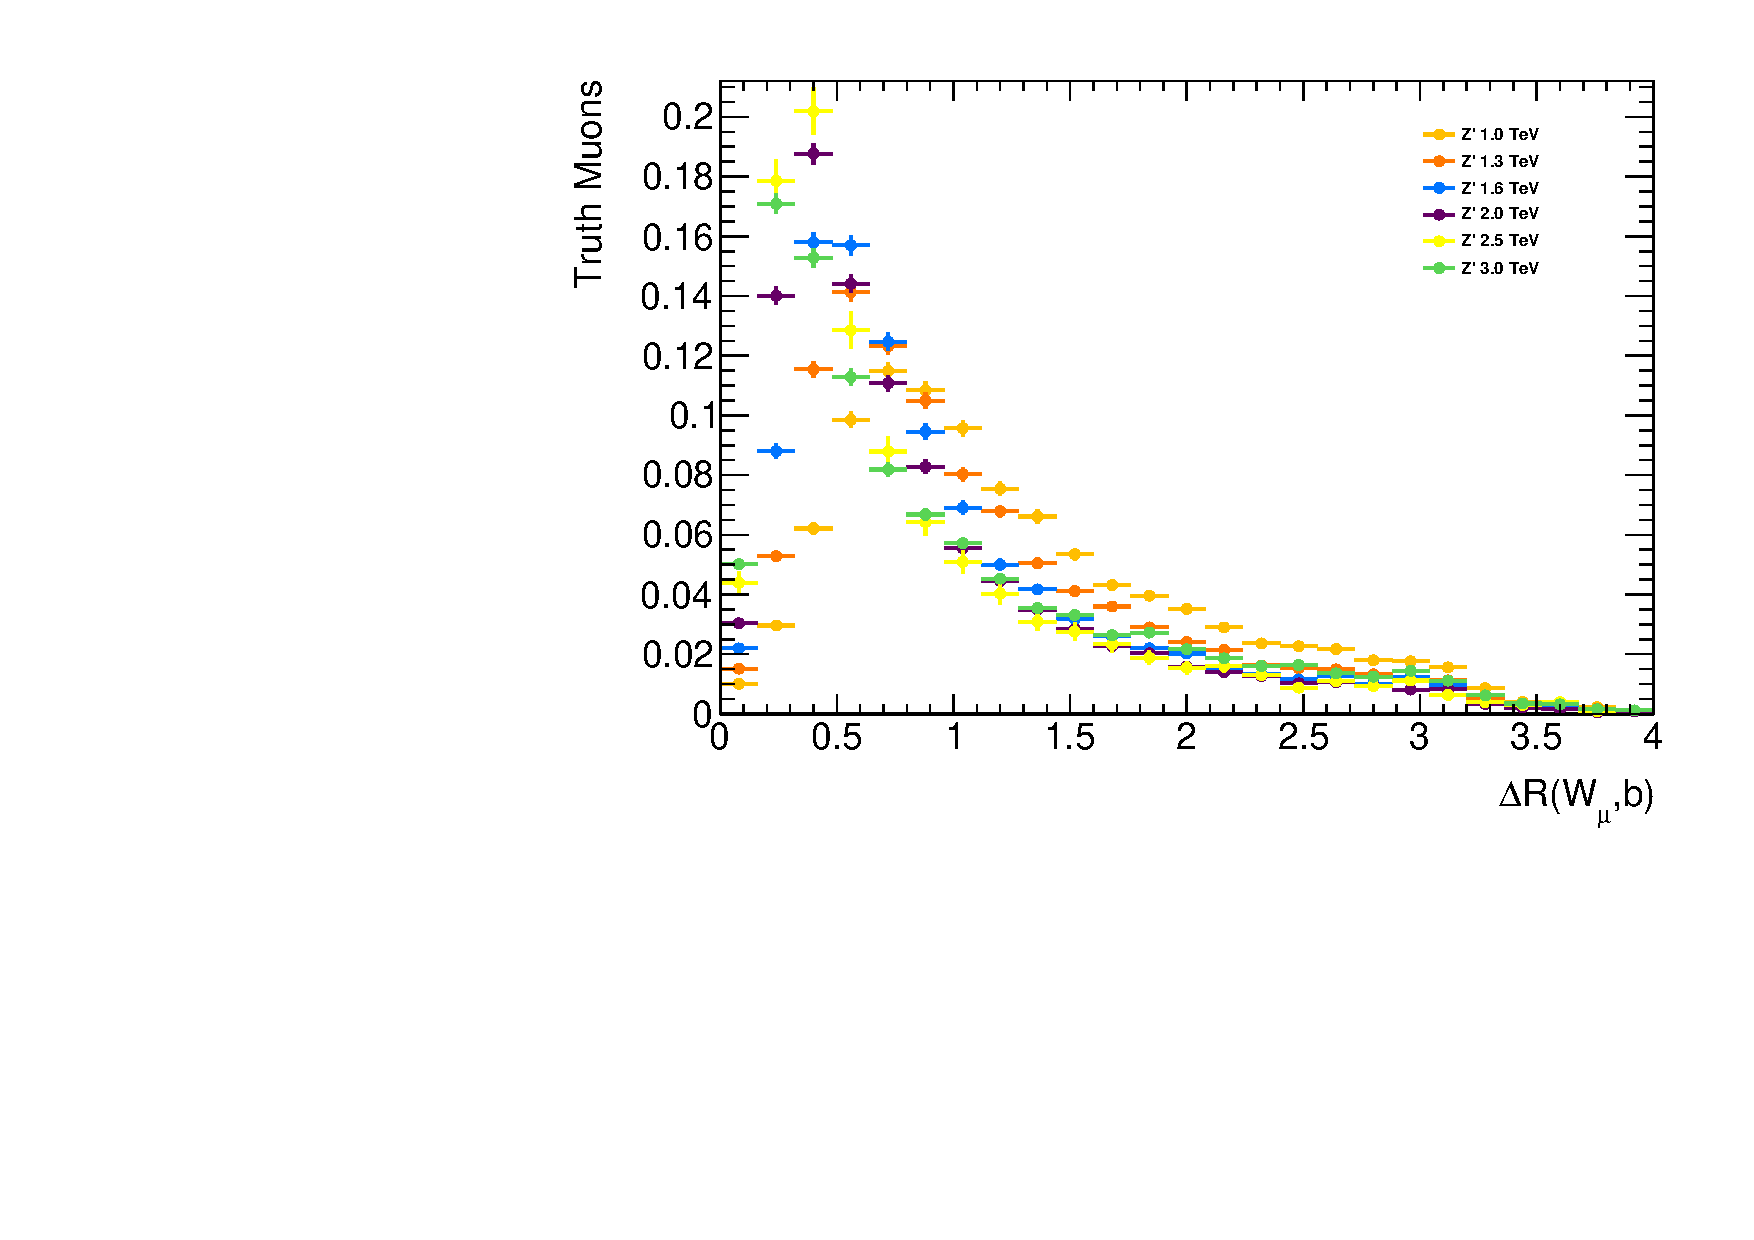
\includegraphics[width=0.75\textwidth]{PartBoosted/Plots/h_trmu_b_dr.pdf}
    \caption{The angular separation (\DeltaR) between the truth \W\ muon and the corresponding $b$-quark for all examined \Zprime\ mass points and non-resonant \ttbar. Uncertainties are omitted for clarity.}\label{fig:ExampleCollimation}
\end{figure}

\begin{figure}[htbp]
  \centering
    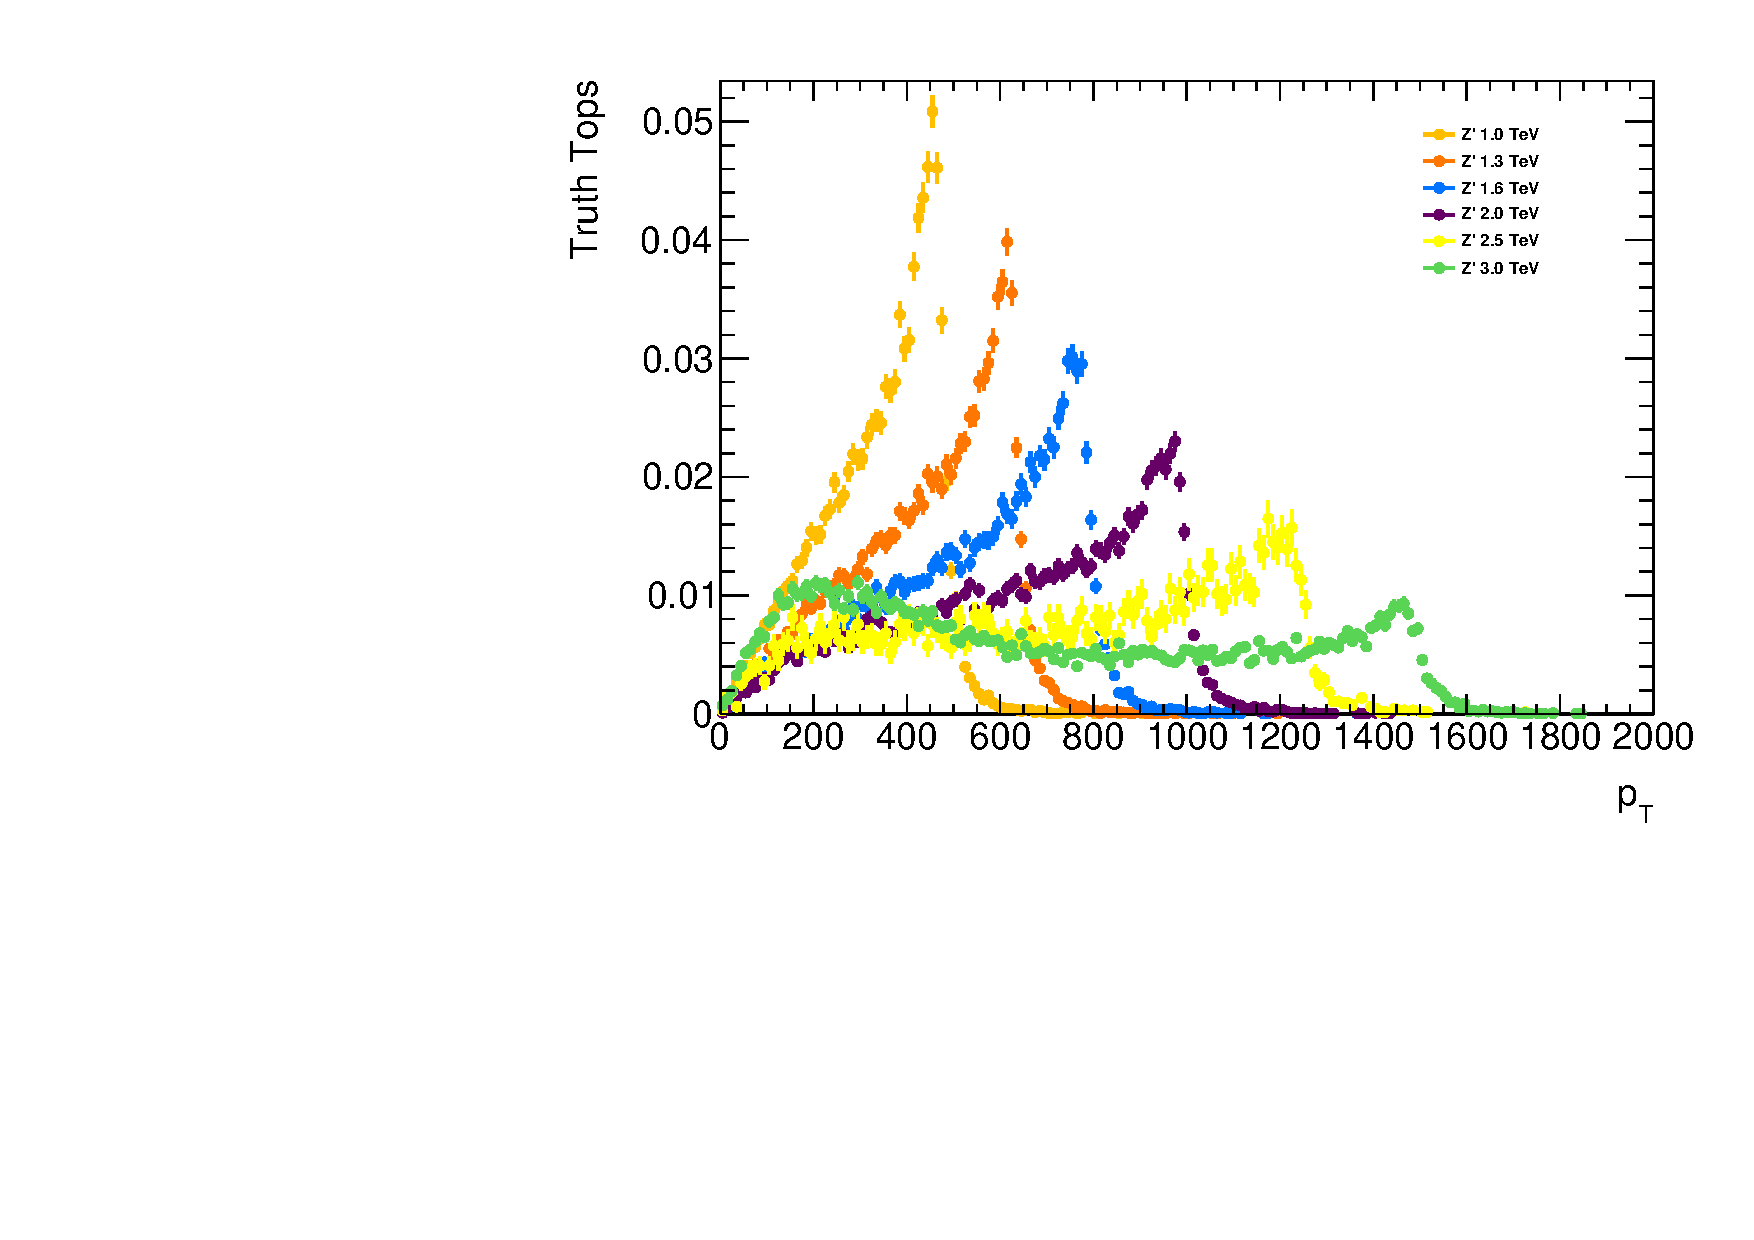
\includegraphics[width=0.75\textwidth]{PartBoosted/Plots/h_trtop_pt.pdf}
    \caption{The transverse momentum of the top/anti-top quarks in the event for all examined \Zprime\ mass points and non-resonant \ttbar. Uncertainties are omitted for clarity.}\label{fig:ExampleBoost}
\end{figure}

\begin{figure}[htbp]
  \centering
    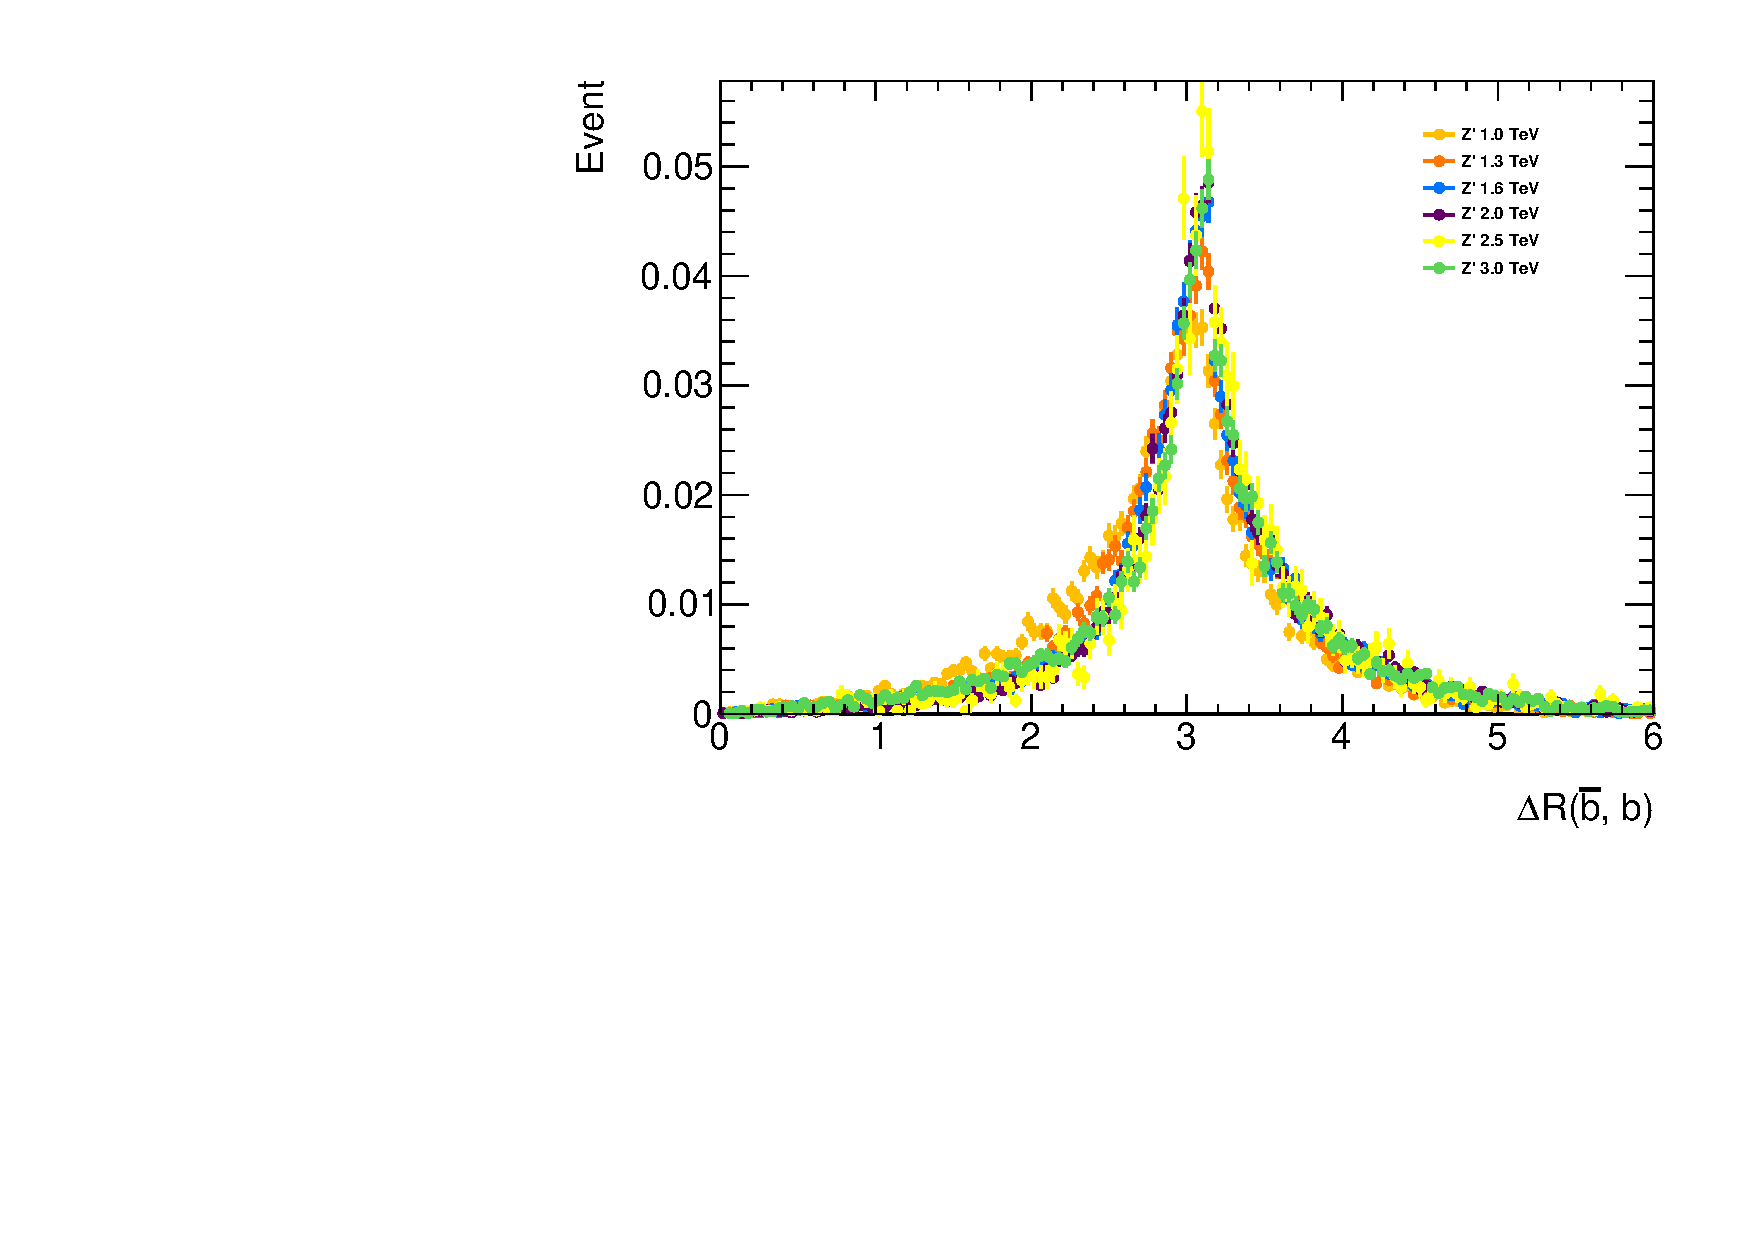
\includegraphics[width=0.75\textwidth]{PartBoosted/Plots/h_b_bbar_dr.pdf}
    \caption{The angular separation (\DeltaR) between the $b$ and $\bar{b}$ in the event for all examined \Zprime\ mass points and non-resonant \ttbar. Uncertainties are omitted for clarity.}\label{fig:ExampleBackToBack}
\end{figure}

\section{Signal muon selection}

Since the signal muon in boosted \ttbar\ events emerge near or within jets, the standard isolation requirements used in SM \ttbar\ analyses erroneously remove \W\ muons. The portion of muons removed increases with collimation and thus \Zprime\ mass. Using the nominal isolation requirement then limits the reach to higher \Zprime\ masses that have yet to be probed.

The ATLAS boosted \ttbar\ resonance analysis proposed an alternative variable to replace the nominal isolation requirement called \emph{mini-isolation} (MI). The absolute MI is defined as the sum of the measured transverse momenta of all tracks in a cone of size $\DeltaR=\kT/\pt^{\ell}$ around the lepton, where \kT\ is an adjustable scale\footnote{For convenience, mini-isolation with a \kT\ value of \SI{10}{\GeV} is referred to as MI10.} and $\pt^{\ell}$ is the momentum of the lepton. This study uses the \emph{relative} MI where the absolute value is scaled by the momentum of the lepton:

\begin{equation}
  \textrm{Rel. MI}=\frac{MI}{\pt^{\ell}}
\end{equation}
%
where $\pt^{\ell}$ is the transverse momentum of the lepton.

MI adapts to the strong collimation of the top products with increasing boost by shrinking the size of the cone for higher boost top quarks. 

The goal of this study is to improve the acceptance at higher \Zprime\ masses by removing the nominal isolation requirement, and instead use the \xsm\ tagger to identify the signal muons.

The performance of the \xsm\ tagger is measured against the conventional isolation criteria, and MI with $\kT=\SI{10}{\GeV}$. The resolved isolation criteria requires the muon to have an $\etcone{20}<\SI{2.5}{\GeV}$ and $\etcone{30}<\SI{4.0}{\GeV}$. For mini-isolation, the lepton is deemed isolated if the $\sum\pt$ is less than \SI{5}{\percent} of the lepton \pt. The \xsm\ tagger operates with the same selection used in Chapter~\ref{ch:Calibration} with the standard operating-point of $\xsd<3.2$.

Two separate selections are applied: one for \xsm\ tagger and one for the resolved isolation and mini-isolation. As mini-isolation and the resolved isolation both use MUID, they share the same set of reconstruction criteria, while the \xsm\ tagger selection is moderately different. All chains require a high-\pt\ muon ($\pt>\SI{20}{\GeV}$) within the pseudorapidity coverage of the ID ($|\eta|<2.5$) that passes the MCP tracking cuts detailed in Appendix~\ref{app:CalibrationMCPCuts}. Mini-isolation and resolved isolation make use of muons reconstructed by the MUID algorithm that pass the so-called \emph{Tight} identification criteria. An additional requirement on the impact parameter ($|z_{0}|<\SI{3.0}{\mm}$) is used to reduce non-prompt muons. The \xsm\ tagger uses the STACO combined algorithm for muon reconstruction with no additional requirements. The cutflows for all three selections are shown in Figure~\ref{fig:BoostedFlowChart}.

The distribution of pseudorapidity for \xsm\ tagged muons, as expected, is similar for all \mzp\ samples as shown in Figure~\ref{fig:BoostedControlSMTeta}. Interestingly, in Figure~\ref{fig:BoostedControlSMTpt}, the average transverse momentum of the \xsm\ muon increases with \mzp\ up to \SI{1.6}{\TeV} then stabilizes for higher masses. This suggests that the $b$-quark takes a larger portion of the top quark momentum above a certain threshold. As expected the angular separation between the \xsm\ tagged muon and the jet in the event decreases with increased \mzp\ as shown in Figure~\ref{fig:BoostedControlSMTdr}. Finally, the \xsd\ distribution is not affected by changes in \mzp\ as shown in Figure~\ref{fig:BoostedControlSMTchi2}. Thus the efficiency of the \xsm\ tagger should be stable through-out the mass range. Similar comments can be made about MI10 muons with regards to their transverse momentum (Figure~\ref{fig:BoostedControlMI10Pt}), pseudorapidity (Figure~\ref{fig:BoostedControlMI10Eta}) and angular separation from the nearest jet (Figure~\ref{fig:BoostedControlMI10Dr}). The size of the cone used in MI is inversely proportional to the lepton \pt. As expected, the cone size distributions are much wider with longer tails at low \mzp\ and more narrow at high \mzp\ as shown in Figure~\ref{fig:BoostedControlMI10Cone}. 

\begin{figure}[htbp]
  \centering
  \begin{subfigure}{0.48\textwidth}
    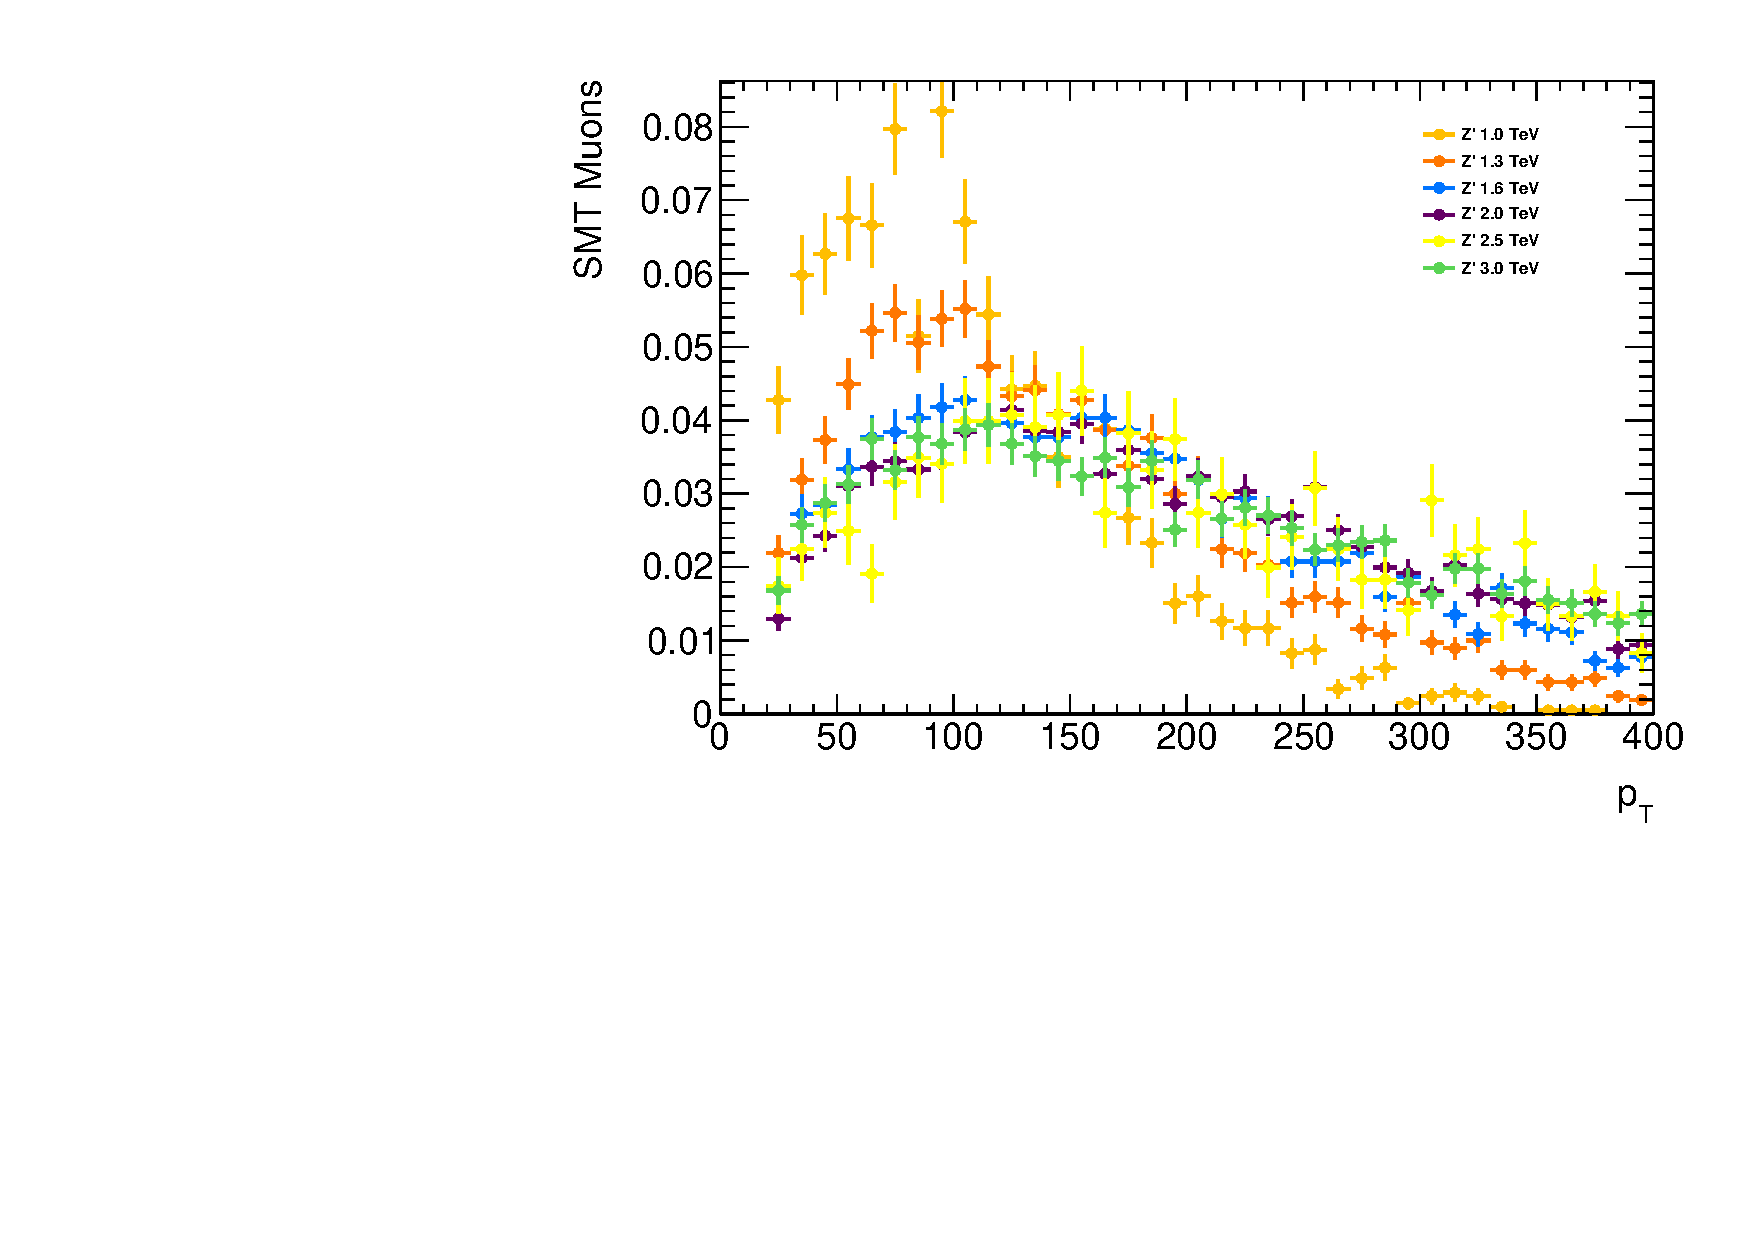
\includegraphics[width=\textwidth]{PartBoosted/Plots/h_smt_pt.pdf}
    \caption{Muon transverse momentum}\label{fig:BoostedControlSMTpt}
  \end{subfigure}
  \begin{subfigure}{0.48\textwidth}
    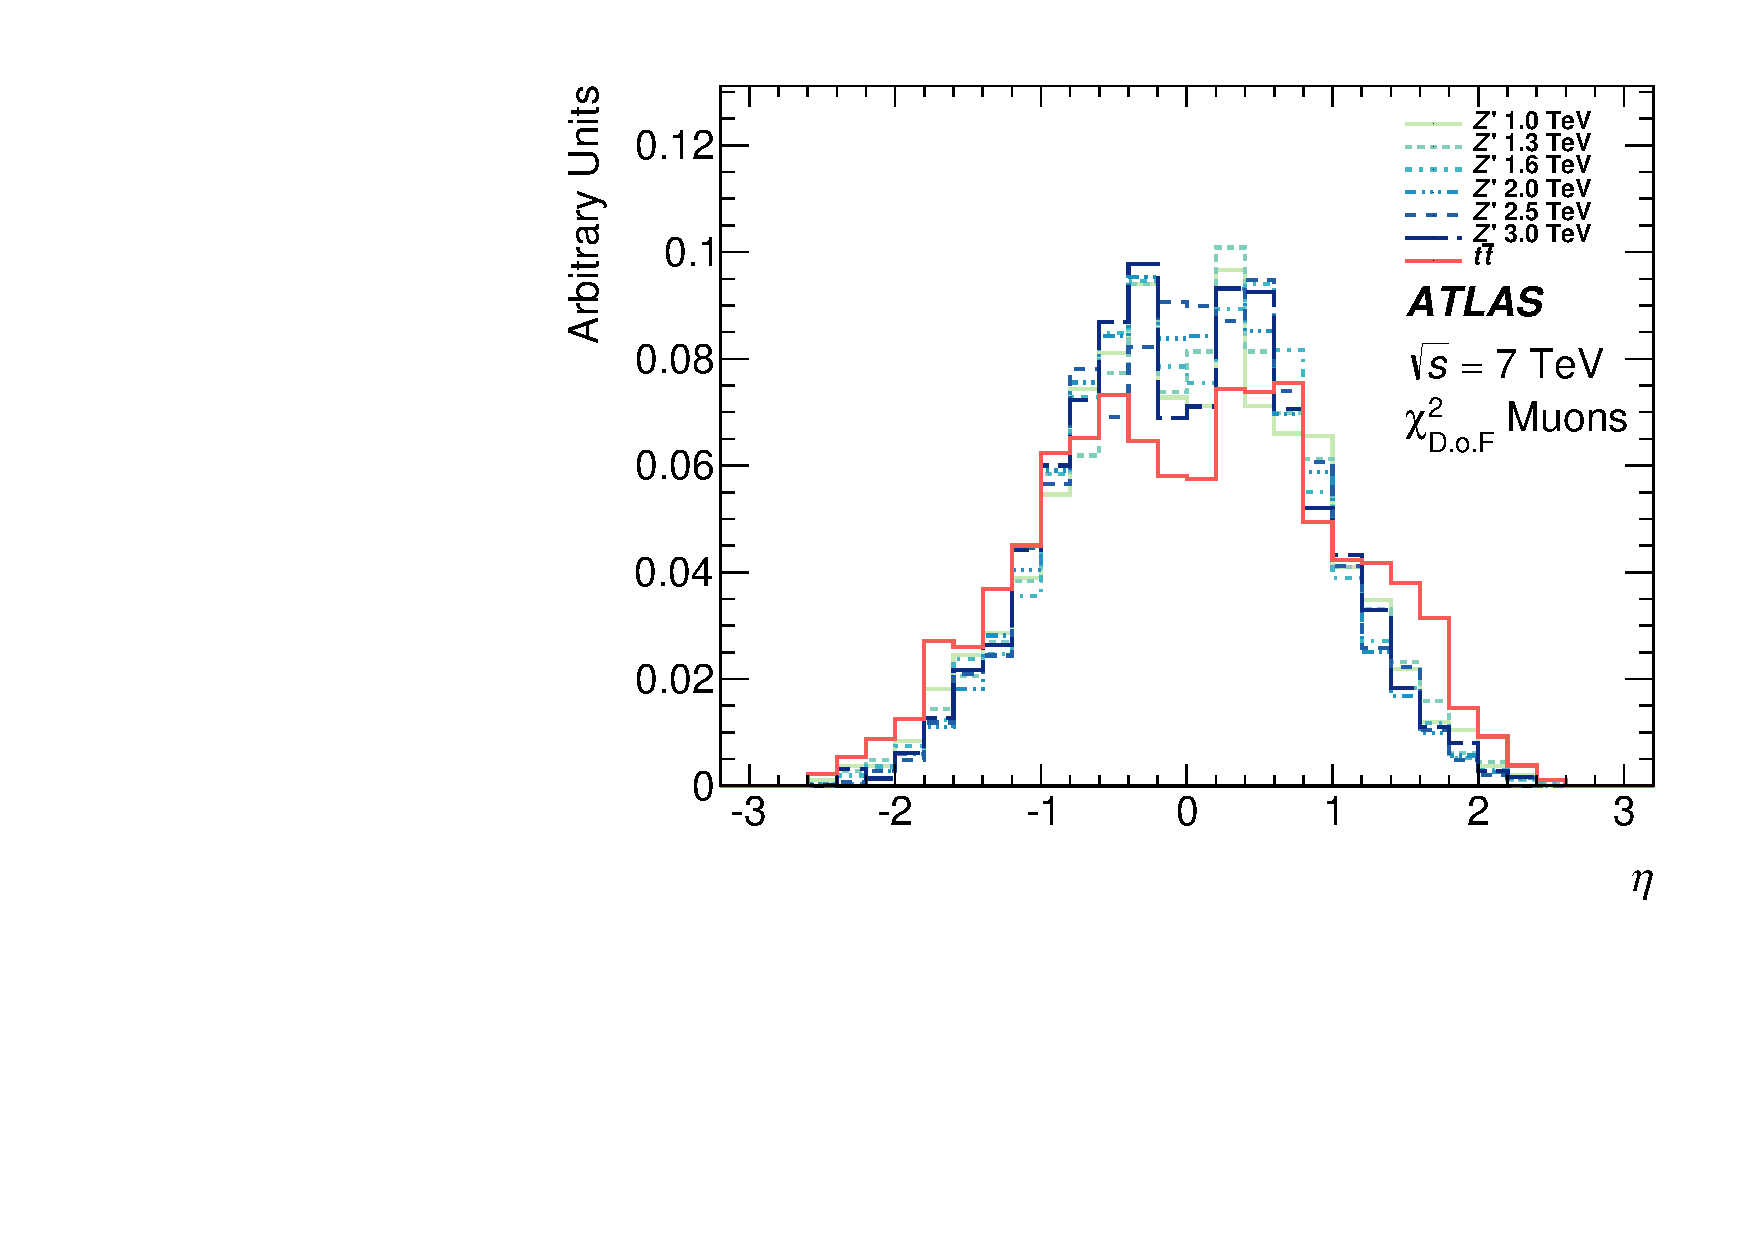
\includegraphics[width=\textwidth]{PartBoosted/Plots/h_smt_eta.pdf}
    \caption{Muon pseudorapidity}\label{fig:BoostedControlSMTeta}
  \end{subfigure}

  \begin{subfigure}{0.48\textwidth}
    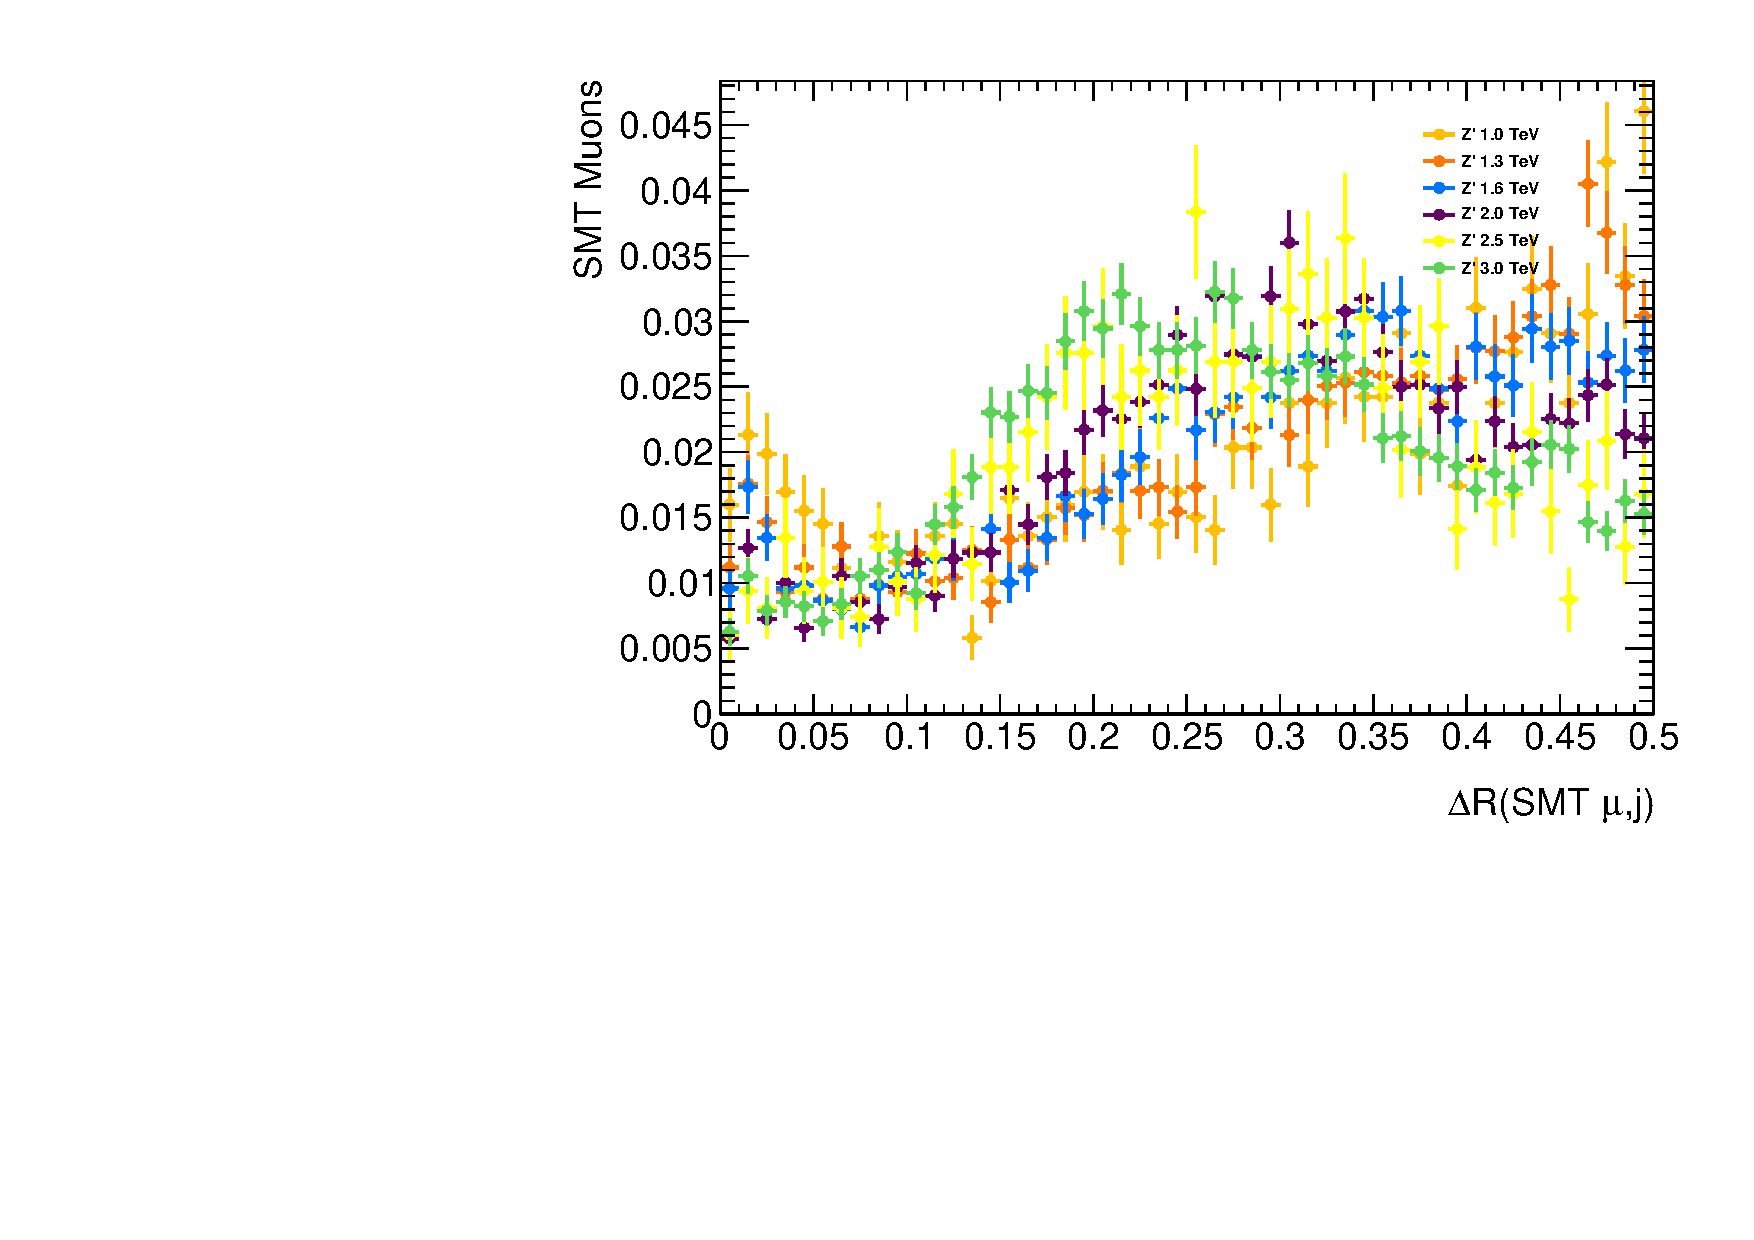
\includegraphics[width=\textwidth]{PartBoosted/Plots/h_smt_jet_dr.pdf}
    \caption{Angular separation from nearest jet}\label{fig:BoostedControlSMTdr}
  \end{subfigure}
  \begin{subfigure}{0.48\textwidth}
    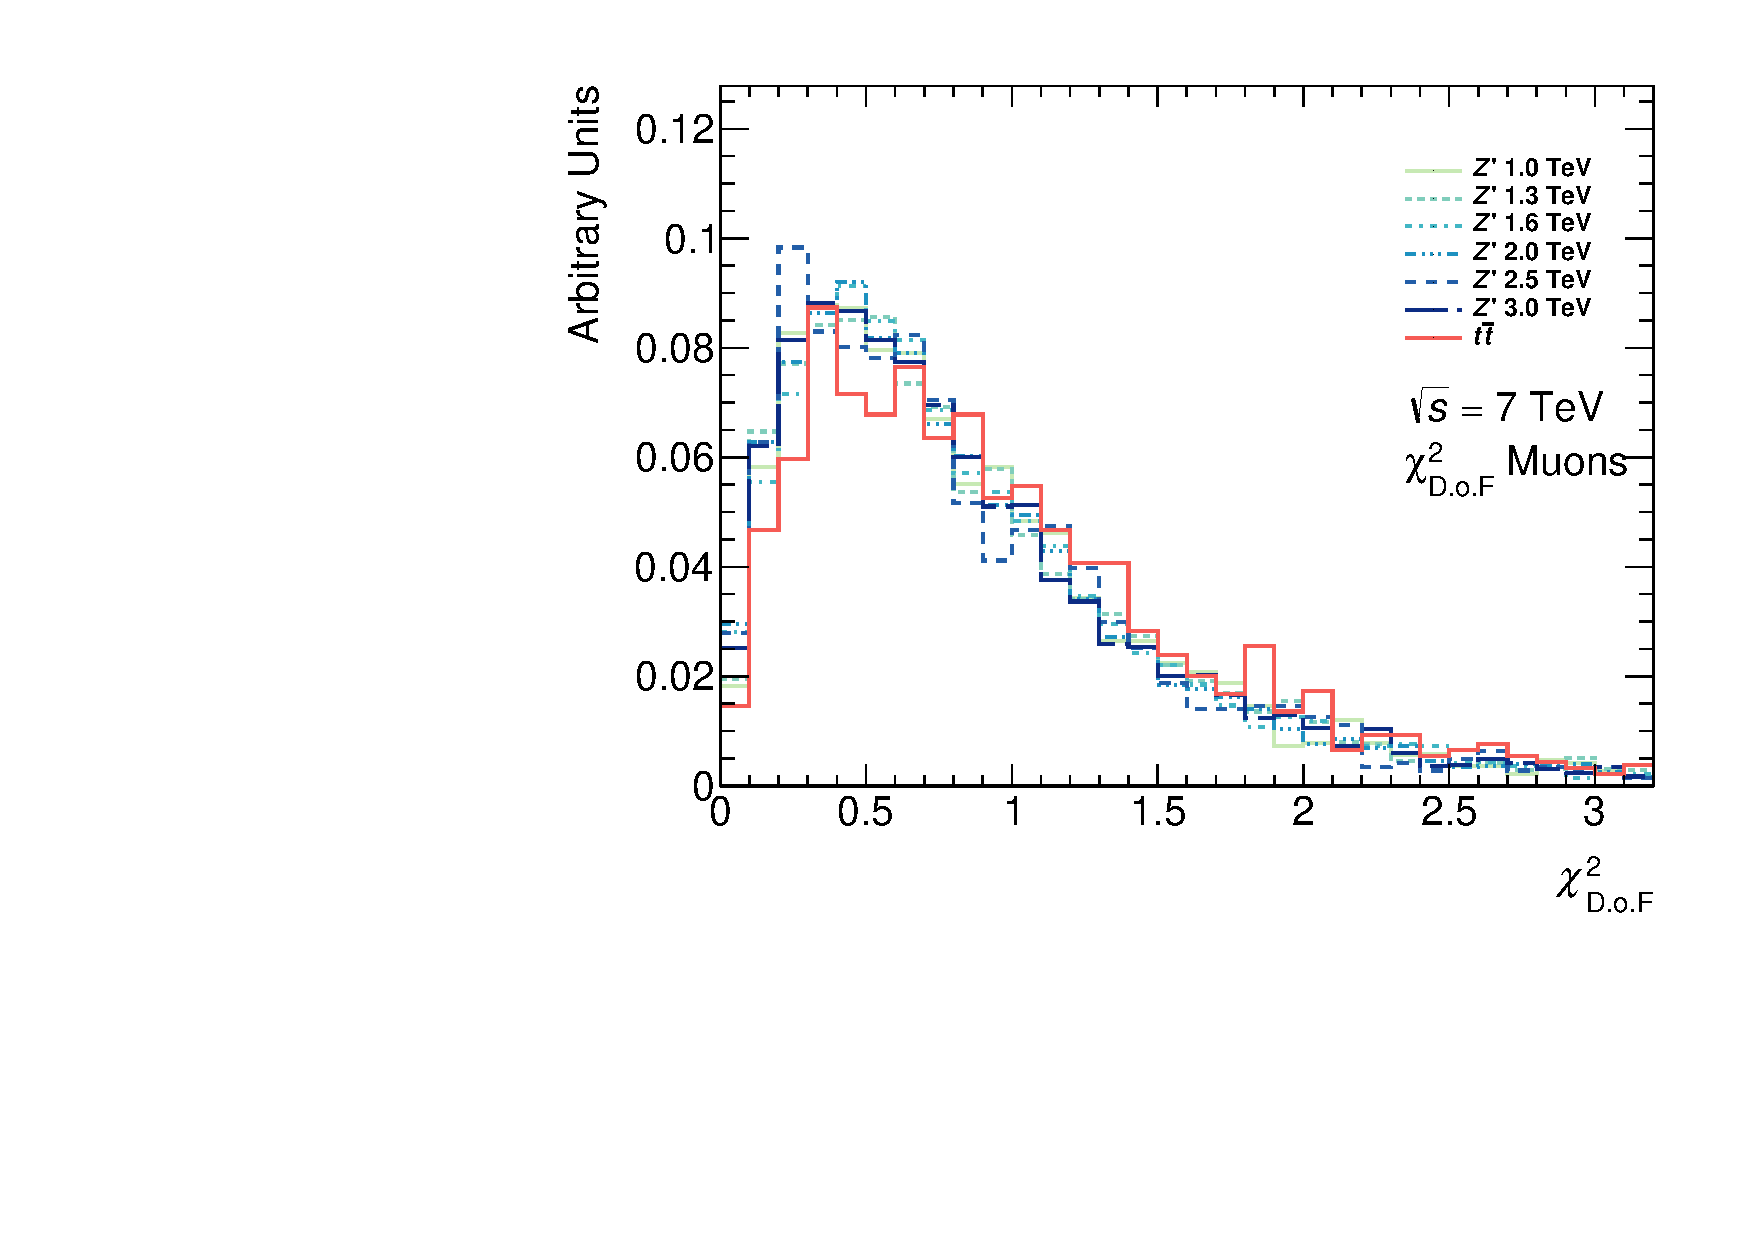
\includegraphics[width=\textwidth]{PartBoosted/Plots/h_smt_chi2.pdf}
    \caption{STACO combined \xsd}\label{fig:BoostedControlSMTchi2}
  \end{subfigure}

  \caption[Distributions for all tested \Zprime\ mass points of the transverse momentum and pseudorapidity of muons which pass the \xsm\ tagger selection, the angular separation between those muons and the nearest jet in the event, and the \xsm\ used in the selection.]{Distributions for all tested \Zprime\ mass points of~\subref{fig:BoostedControlSMTpt} the transverse momentum and~\subref{fig:BoostedControlSMTeta} pseudorapidity of muons which pass the \xsm\ tagger selection, the~\subref{fig:BoostedControlSMTdr} angular separation between those muons and the nearest jet in the event, and~\subref{fig:BoostedControlSMTchi2} the \xsm\ used in the selection. All distributions normalized to unit area.}\label{fig:BoostedControlSMT}
\end{figure}

\begin{figure}[htbp]
  \centering
  \begin{subfigure}{0.48\textwidth}
    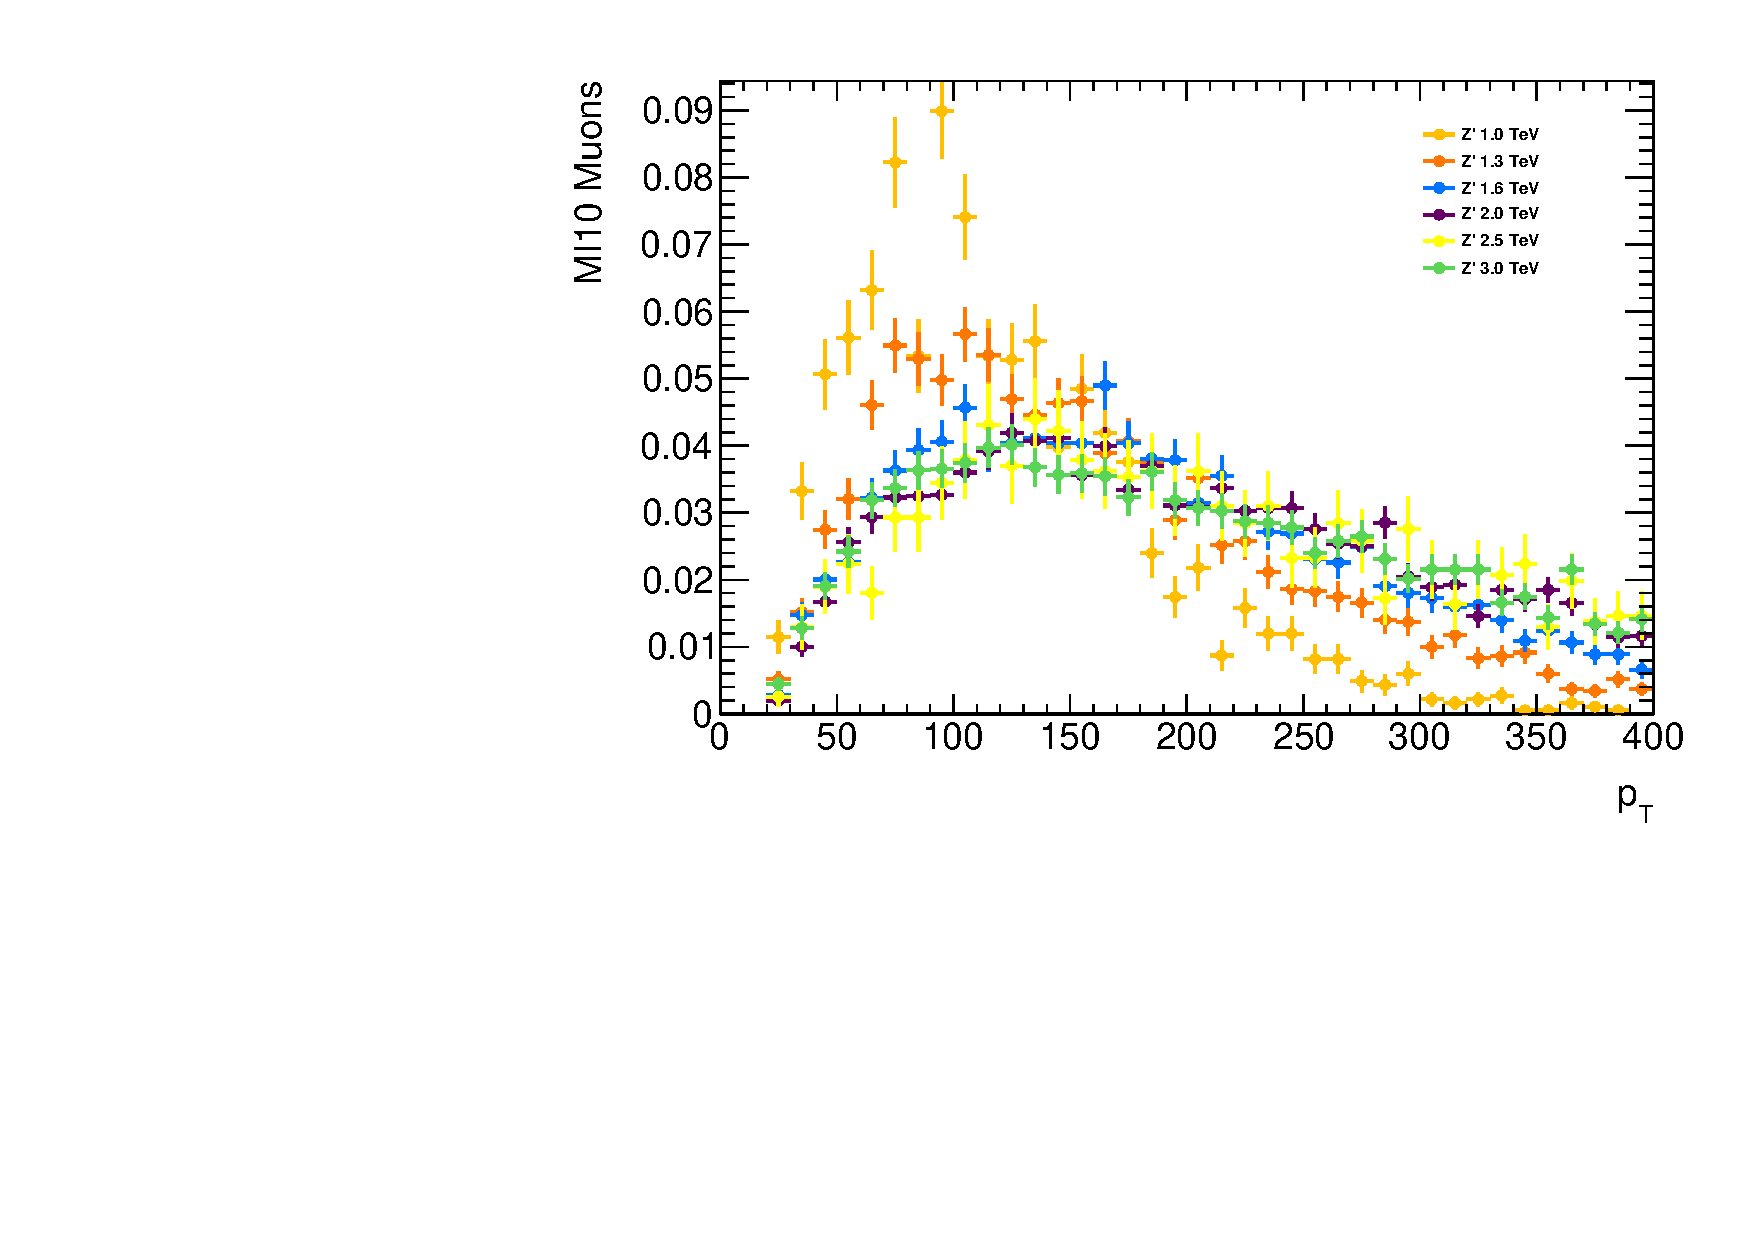
\includegraphics[width=\textwidth]{PartBoosted/Plots/h_mi10_pt.pdf}
    \caption{Muon transverse momentum}\label{fig:BoostedControlMI10Pt}
  \end{subfigure}
  \begin{subfigure}{0.48\textwidth}
    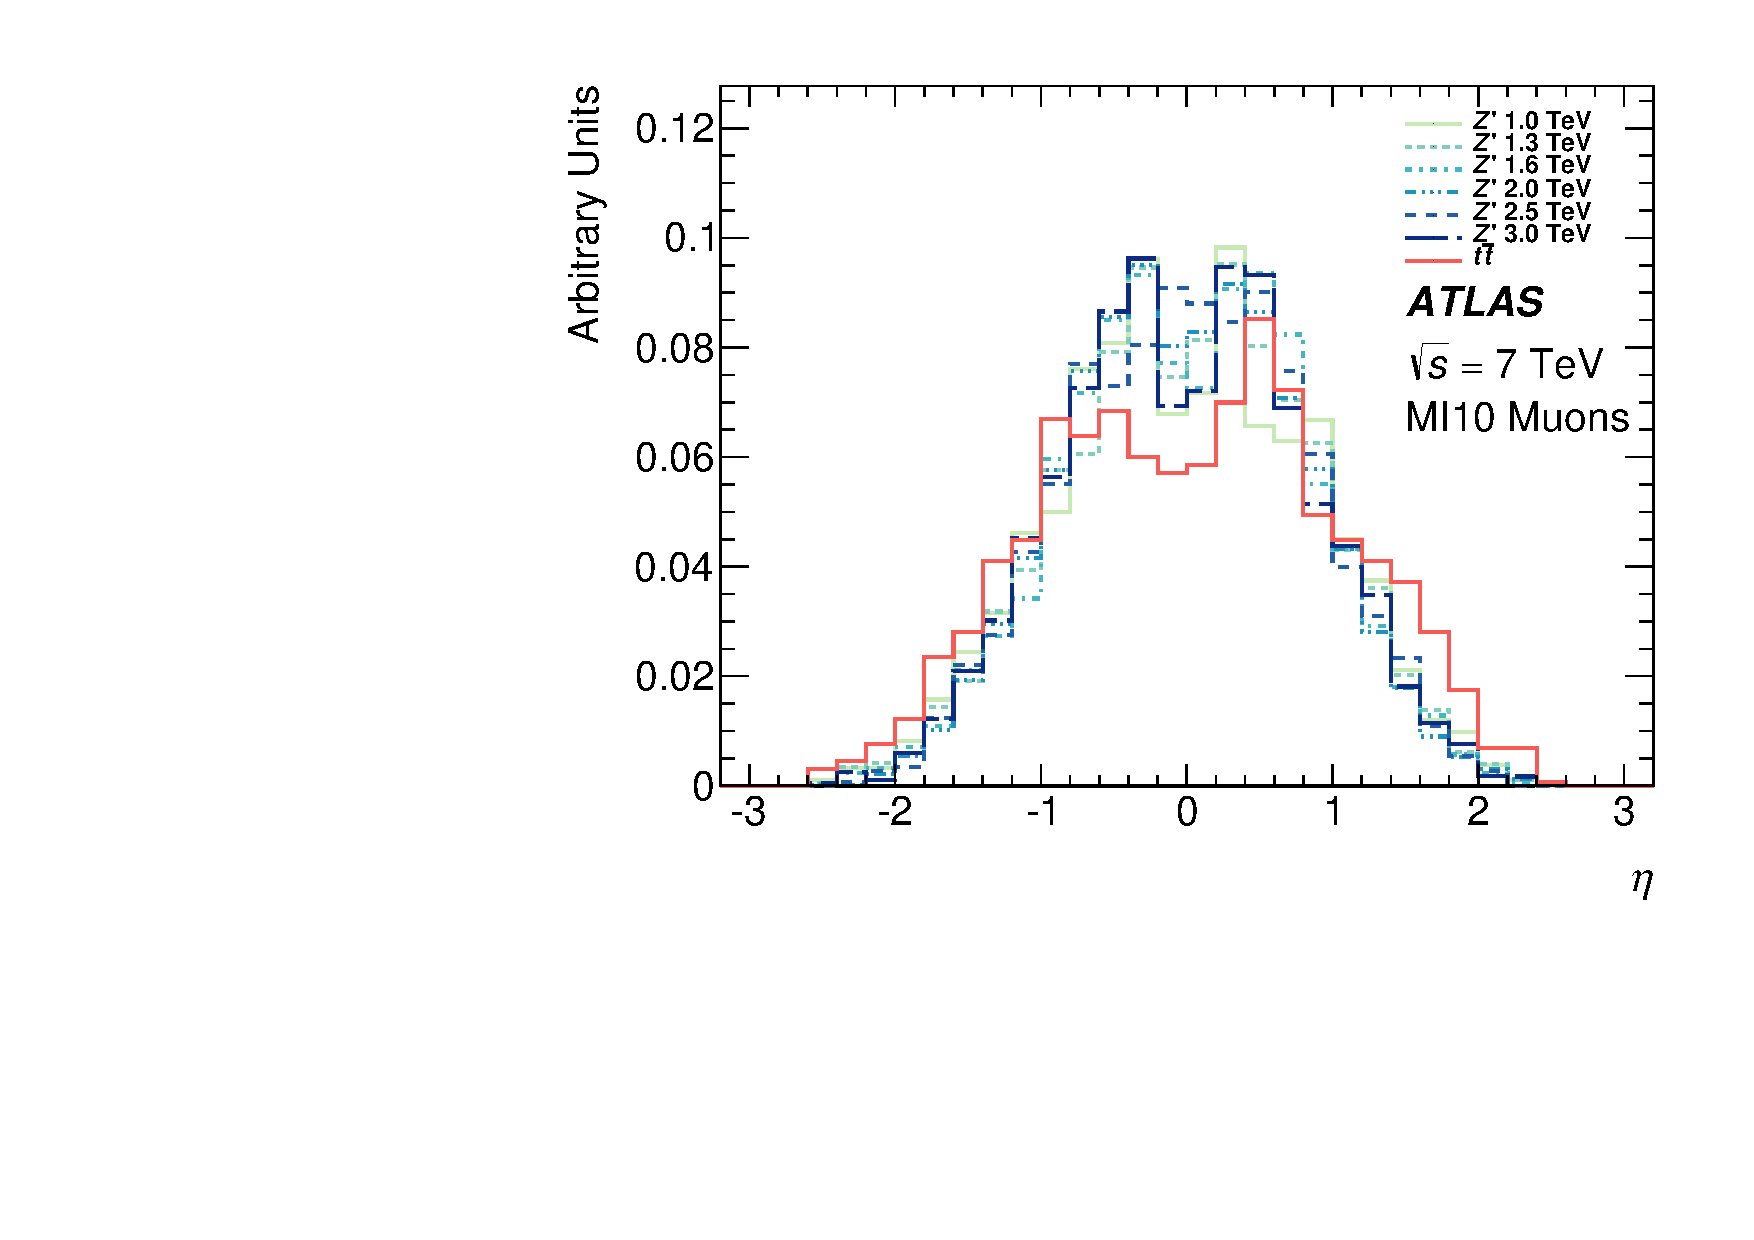
\includegraphics[width=\textwidth]{PartBoosted/Plots/h_mi10_eta.pdf}
    \caption{Muon pseudorapidity}\label{fig:BoostedControlMI10Eta}
  \end{subfigure}

  \begin{subfigure}{0.48\textwidth}
    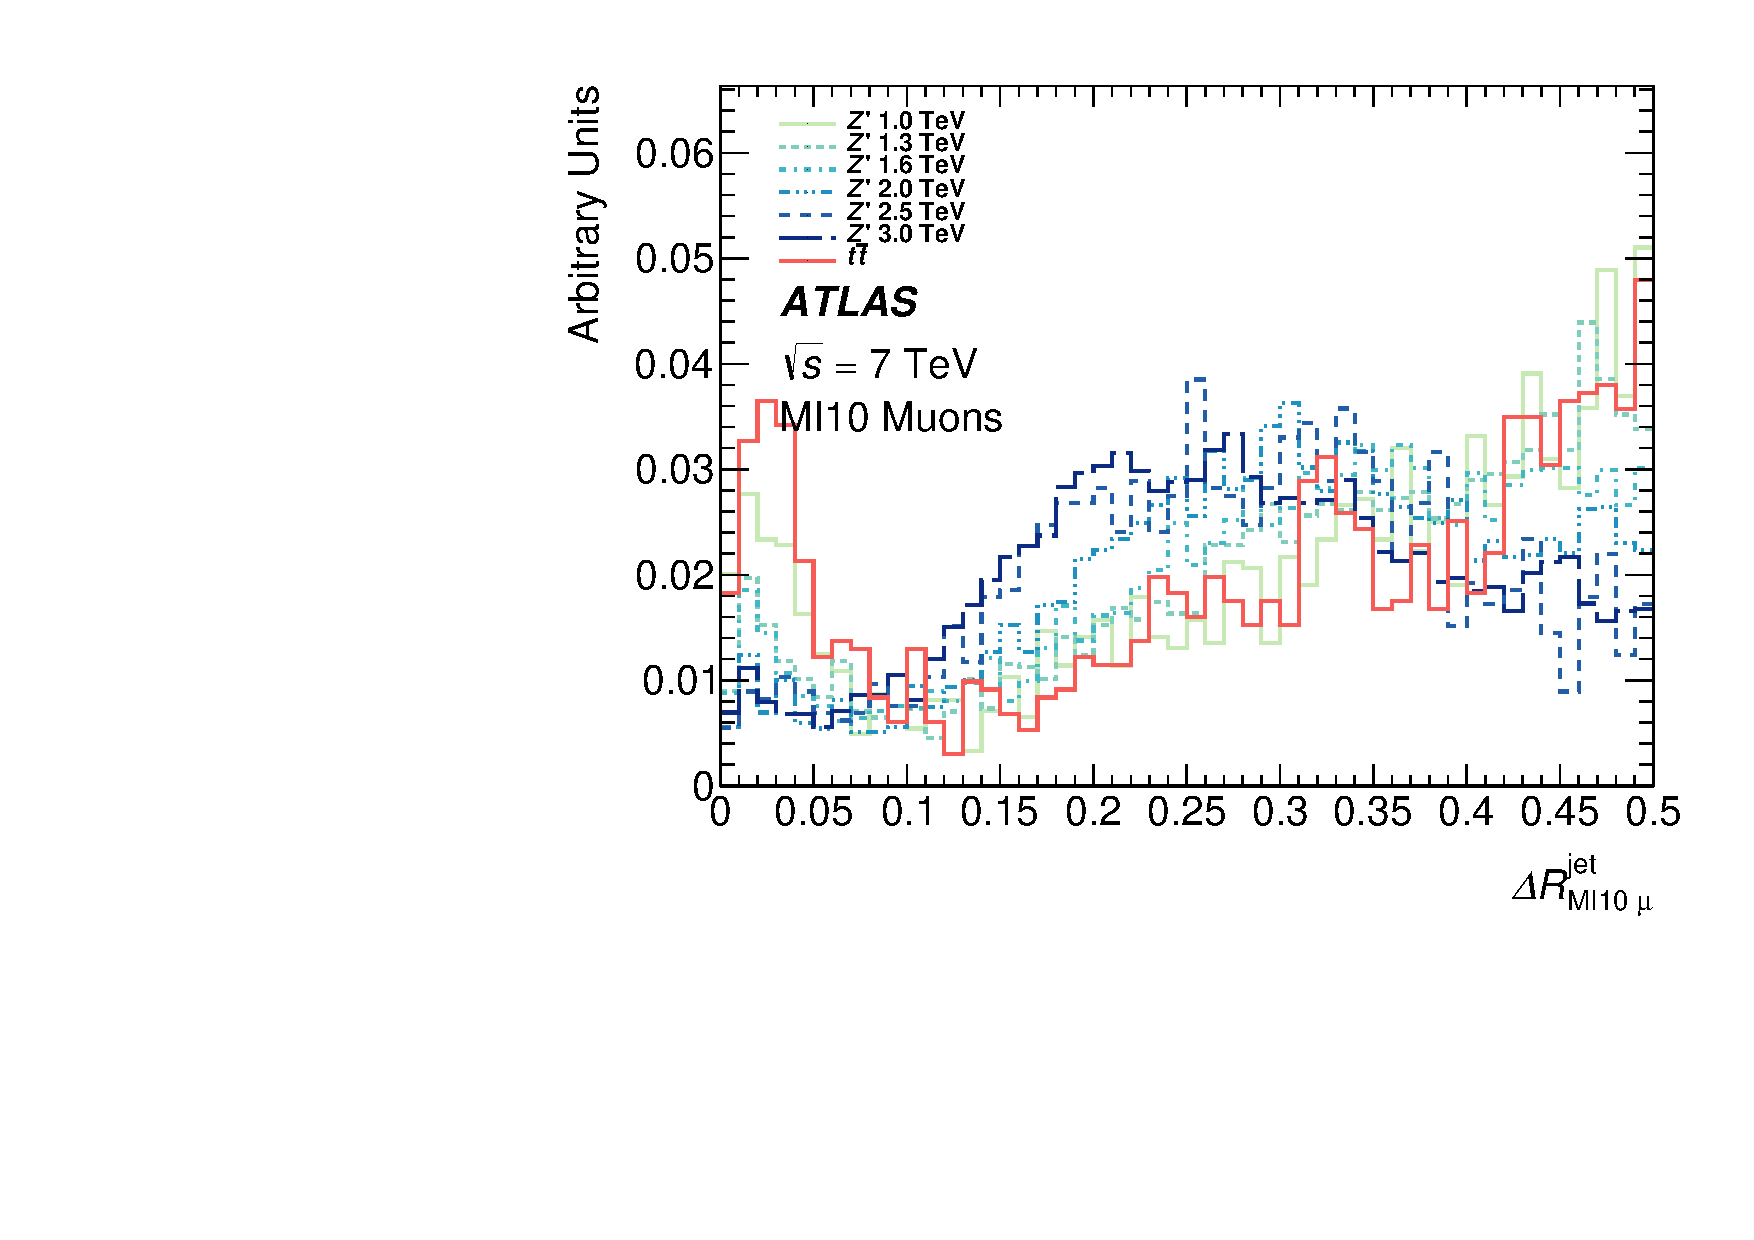
\includegraphics[width=\textwidth]{PartBoosted/Plots/h_mi10_jet_dr.pdf}
    \caption{Angular separation from nearest jet}\label{fig:BoostedControlMI10Dr}
  \end{subfigure}
  \begin{subfigure}{0.48\textwidth}
    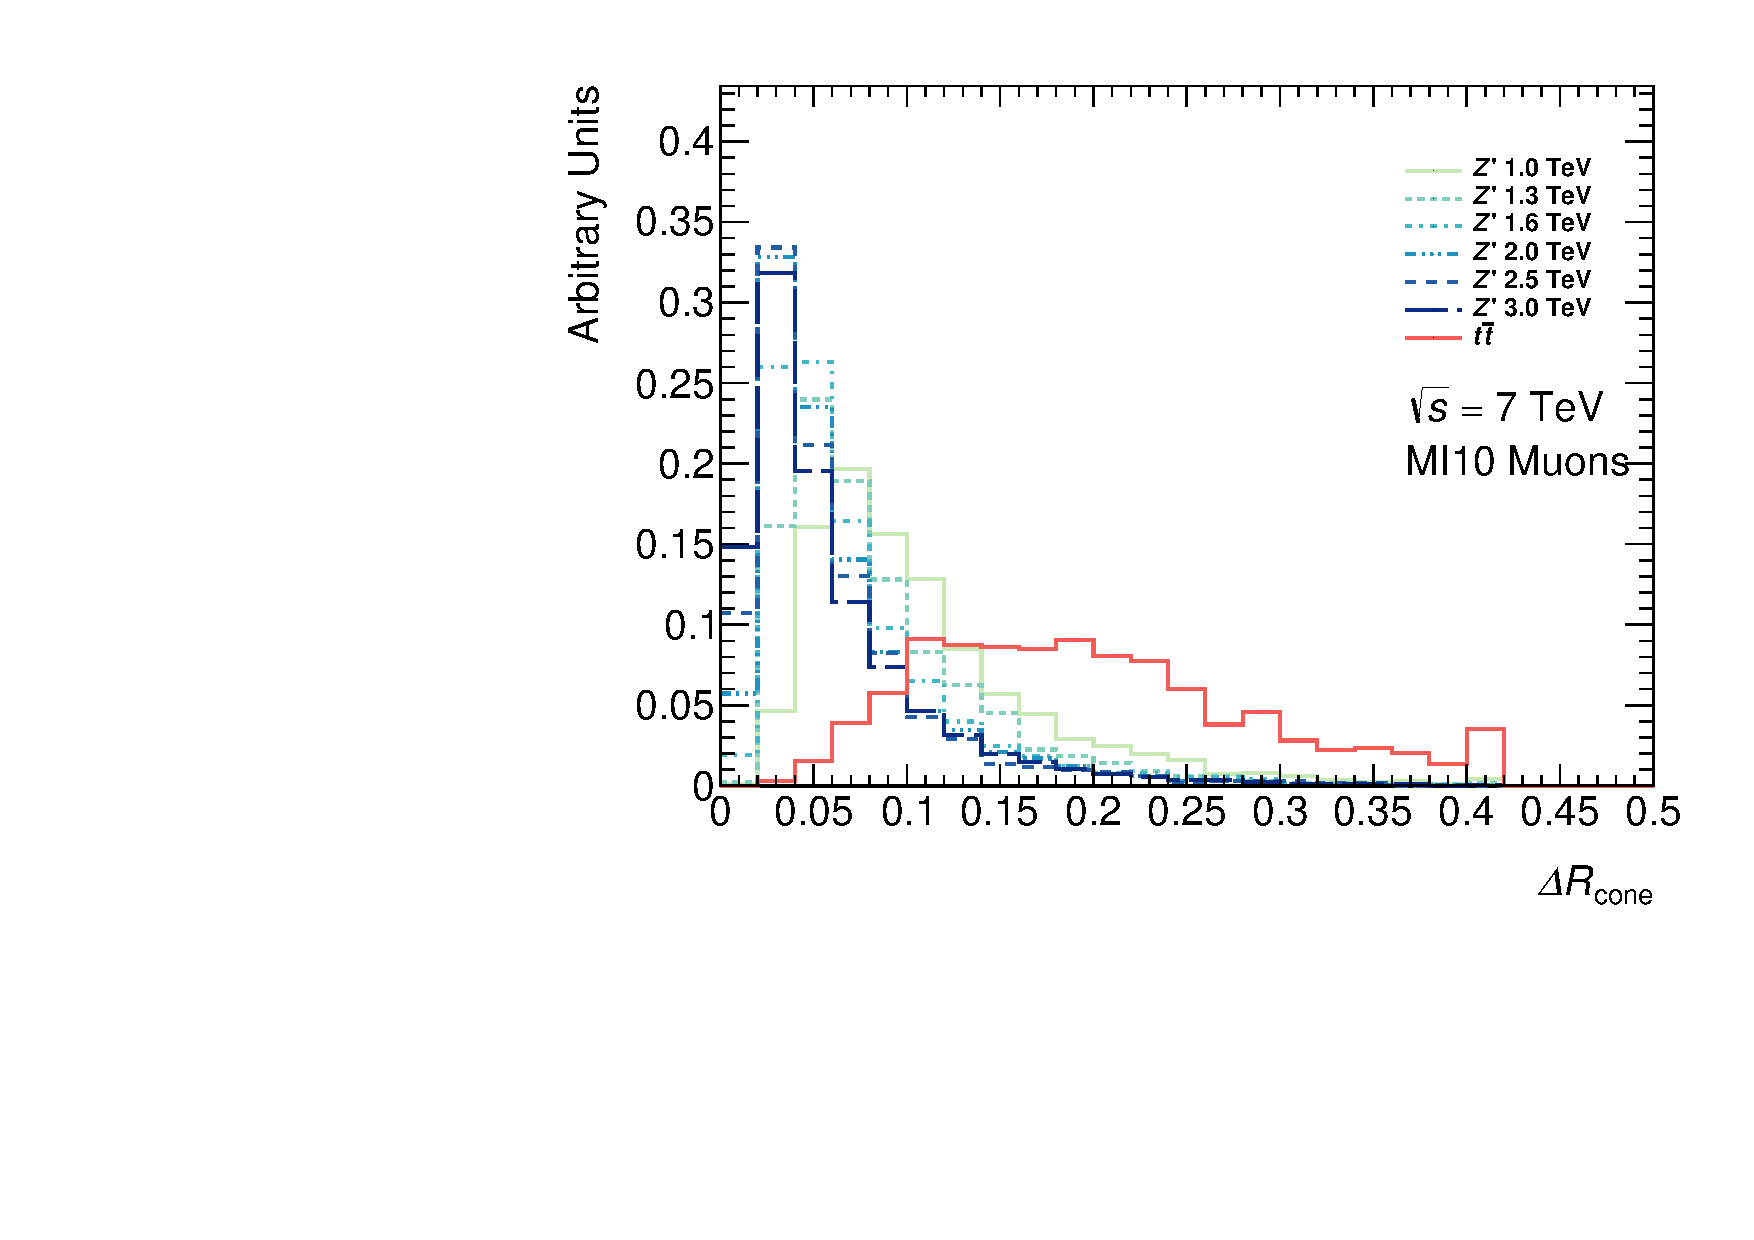
\includegraphics[width=\textwidth]{PartBoosted/Plots/h_mi10_coneSize.pdf}
    \caption{Size of isolation cone}\label{fig:BoostedControlMI10Cone}
  \end{subfigure}

  \caption[Distributions for all tested \Zprime\ mass points of the transverse momentum and pseudorapidity of muons which pass the MI10 selection, the angular separation between those muons and the nearest jet in the event, and the cone size used in the selection.]{Distributions for all tested \Zprime\ mass points of~\subref{fig:BoostedControlMI10Pt} the transverse momentum and~\subref{fig:BoostedControlMI10Eta} pseudorapidity of muons which pass the MI10 selection, the~\subref{fig:BoostedControlMI10Dr} angular separation between those muons and the nearest jet in the event, and~\subref{fig:BoostedControlMI10Cone} the cone size used in the selection. All distributions normalized to unit area.}\label{fig:BoostedControlMI10}
\end{figure}

\section{Efficiency definition}\label{sec:BoostedEfficiencyDefinition}

The efficiency measurement was designed to provide an accurate representation of the performance of the \xsm\ tagger and a fair comparison with mini-isolation. Additional sources of inefficiency such as muon reconstruction are separated out into an additional efficiency which is also quoted. See Figure~\ref{fig:BoostedFlowChart} for a summary of the efficiency measurement.

\begin{figure}[htpb]
  \centering
    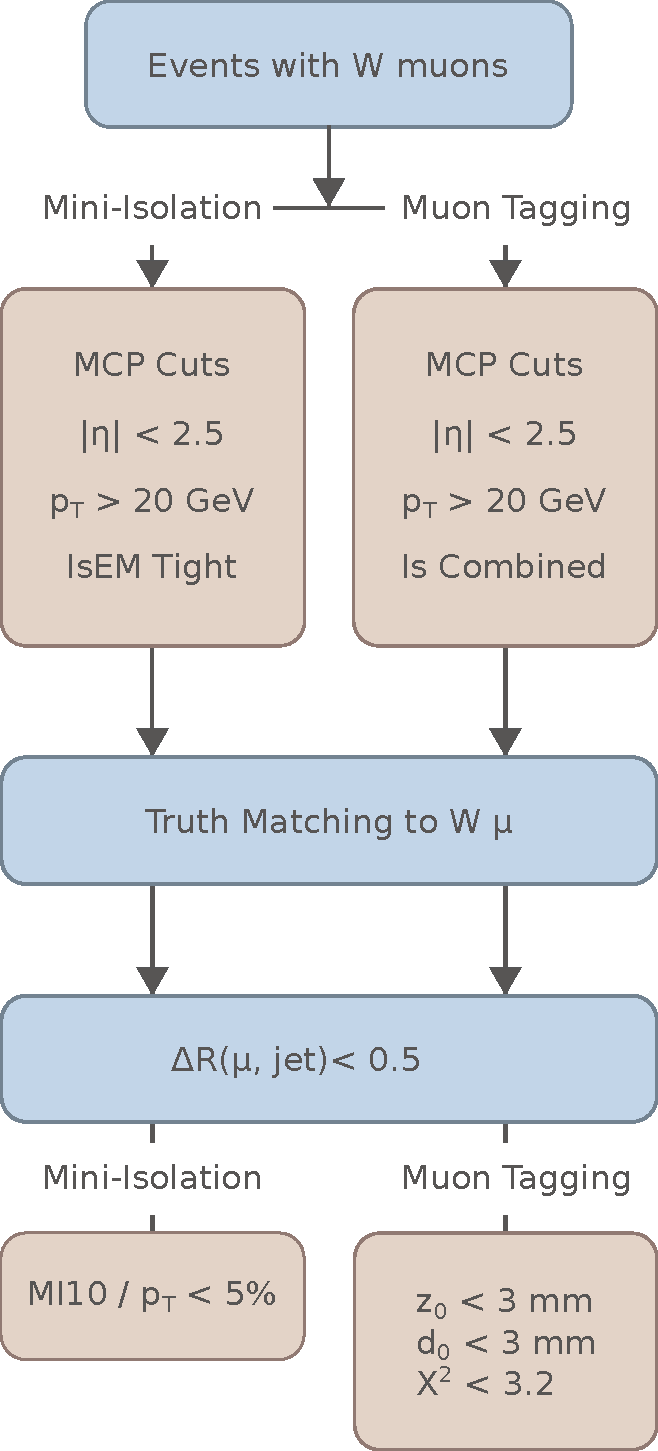
\includegraphics[width=0.85\textwidth]{PartBoosted/Plots/FlowChart.pdf}
    \caption{Structure of the efficiency measurement including both cut-flows.}\label{fig:BoostedFlowChart}
\end{figure}

Firstly, events where a \W\ boson decays into a muon are selected using truth information. These events are then used to measure the efficiency. Note that at each stage the denominator is the numerator of the previous efficiency. Thus the complete efficiency is given by the product of all the efficiency components. This allows for an estimation of the number of \W\ muons that would be selected.

First, the truth \W\ muons are matched to STACO/MUID muons if the angular separation (\DeltaR) between them is less than $0.0015$. The matching efficiency is defined as:

\begin{equation}
  \eff{\textrm{match}}{} = \frac{\textrm{STACO/MUID muons matched to truth \W\ muon}}{\textrm{Truth \W\ muons}}
\end{equation}

The selections then diverge and the two sets of reconstruction cuts described earlier are applied independently with an efficiency defined as:

\begin{equation}
  \eff{\textrm{reco}}{} = \frac{\textrm{STACO/MUID muons that pass reconstruction cuts}}{\textrm{STACO/MUID muons matched to truth \W\ muon}}
\end{equation}

Next the muons are required to be within $\DeltaR<0.5$ from a jet. The impetus behind the analysis is to probe highly boosted events exploiting the capabilities of \xsm\ tagging. This selection ensures that the muons available for \xsm\ tagging are indeed close to a jet. This selection also has an efficiency associated with it defined as:

\begin{equation}
  \eff{\textrm{non-iso}}{}=\frac{\textrm{Muons with $\DeltaR^{\textrm{jet}}_{\mu}<0.5$}}{\textrm{STACO/MUID muons that pass reconstruction cuts}}
\end{equation}

The final step is the application of either the mini-isolation selection or the \xsm\ tagger selection discussed above. These selections are associated with the final and most interesting sets of efficiencies, defined as:

\begin{equation}
  \eff{\xsm\textrm{/MI10/Res.}}{}= \frac{\textrm{Muons which pass }\xsm\textrm{/MI10/Res. selection}}{\textrm{Muons with $\DeltaR^{\textrm{jet}}_{\mu}<0.5$}}
  \label{eq:BoostedMI}
\end{equation}

In the nominal analysis described in~\cite{Boosted:ATLASExclusion7TeV} muons which are within $\DeltaR=0.1$ of the jet would be removed. The goal of the analysis is to exploit the \xsm\ tagger to accept additional events where the signal muon emerges very close to the jet axis, thus overlap removal~\footnote{True objects may be reconstructed as two different objects, such as an electron and jet. Overlap removal is the act of selecting the true object from two overlapping reconstructed objects.} is not traditionally part of the \xsm\ tagging selection. Two sets of efficiencies are provided here: one without overlap (defined in Eq~\ref{eq:BoostedMI}) and one with overlap removal, defined below

\begin{equation}
  \eff{\xsm\textrm{/MI10/Res.+overlap}}{} = \frac{\textrm{Muons which pass the \xsm/MI10/Res. selection with $\DeltaR^{\textrm{jet}}_{\mu}>0.1$}}{\textrm{Muons with $\DeltaR^{\textrm{jet}}_{\mu}<0.5$}}
\end{equation}

\section{Results}

The results of the reconstruction portion of the analysis chains are summarized in Table~\ref{tab:BoostedRecoSTACO} for the \xsm\ chain and in Table~\ref{tab:BoostedRecoMUID} for the mini-isolation chain. The matching efficiency (\eff{\textrm{match}}{}) is stable with respect to \Zprime\ mass for both MUID and STACO, meaning that both algorithms are able to reconstruct the signal muon irrespective of boost. Within the uncertainty neither algorithm appears to be better than other at reconstruction of these muons. The efficiencies of both reconstruction selections (\eff{\textrm{reco}}{}) are compatible within uncertainties and appear to be slightly lower at low \Zprime\ mass, likely due to the \pt\ requirement on the muon. Finally, the collimation effect due to increased boost is clearly visible in the non-isolation efficiency. A marked increase with \Zprime\ mass is noted as the products of the top quarks get pushed closer together. Note that the results obtained at $\mzp=\SI{2.5}{\TeV}$ suffer from lack of data compared to the other mass points. Once again, this effect those not appear to affect one reconstruction algorithm more than the other and the efficiencies are compatible within uncertainty.

% STACO Reconstruction Results
\begin{table}[htbp]
  \centering
  \begin{tabular}{@{}%
                  S[table-format=4] %
                  S[table-format=5] %
                  *{3}{S[table-format=2.1(1)]} %
                  @{}}
    \toprule
    {\mzp\ [\si{\GeV}]} & $N^{\textrm{from }W}_{\textrm{muons}}$ & \multicolumn{3}{c}{Efficiency [\si{\percent}]} \\
    \cmidrule{3-5}
    && $\eff{\textrm{match}}{\textrm{STACO}}$ & $\eff{\textrm{reco}}{\textrm{STACO}}$ & $\eff{\textrm{non-iso.}}{\textrm{STACO}}$ \\
    \midrule
    1000 & 13700(100) & 91.3(2) & 85.5(3) & 20.4(4)  \\
    1300 & 15500(100) & 92.0(2) & 86.4(3) & 31.8(4)  \\
    1600 & 13400(100) & 91.9(2) & 87.5(3) & 42.4(5)  \\
    2000 & 15300(100) & 92.1(2) & 87.9(3) & 51.3(5)  \\
    2500 & 3310(60)   & 91.9(5) & 88.1(6) & 57.7(10) \\
    3000 & 15300(100) & 91.8(2) & 87.5(3) & 51.4(5)  \\
    \bottomrule
  \end{tabular}
  \caption{Results of constructing the muon sample used to estimate the efficiency of the \xsm\ tagger. Uncertainty is statistical only.}\label{tab:BoostedRecoSTACO}
\end{table}

% MUID Reconstruction Results
\begin{table}[htbp]
  \centering
  \begin{tabular}{@{}
                  S[table-format=4] %
                  S[table-format=5] %
                  S[table-format=2.1(1)] %
                  S[table-format=2.1(1)] %
                  S[table-format=2.1(1)] %
                  @{}}
  \toprule
  {\mzp\ [\si{\GeV}]} & $N^{\textrm{from }W}_{\textrm{muons}}$ & \multicolumn{3}{c}{Efficiency [\si{\percent}]} \\
  \cmidrule{3-5}
  && $\eff{\textrm{match}}{\textrm{MUID}}$ & $\eff{\textrm{reco}}{\textrm{MUID}}$ & $\eff{\textrm{non-iso}}{\textrm{MUID}}$ \\
  \midrule
  1000 & 13700(100) & 91.7(2) & 86.6(3) & 20.3(4) \\
  1300 & 15500(100) & 92.2(2) & 87.6(3) & 31.9(4) \\
  1600 & 13400(100) & 92.2(2) & 88.7(3) & 42.2(5) \\
  2000 & 15300(100) & 92.5(2) & 88.8(3) & 51.2(4) \\
  2500 & 3310(60)   & 92.2(5) & 89.1(7) & 57.9(9) \\
  3000 & 15300(100) & 92.1(2) & 88.5(3) & 51.2(4) \\
  \bottomrule  
  \end{tabular}
  \caption[Results of constructing the muon sample used to estimate the efficiency of mini-isolation and resolved isolation.]{Results of constructing the muon sample used to estimate the efficiency of mini-isolation and resolved isolation. The uncertainty is statistical only.}\label{tab:BoostedRecoMUID}
\end{table}

The efficiency of the resolved isolation is low and decreases with increasing boost to \SI{18}{\percent} at $\mzp=\SI{3.0}{\TeV}$ as shown in Table~\ref{tab:BoostedFinalResolved}, highlighting the need for a better isolation requirement.

\begin{table}[htbp]
\centering
  \begin{tabular}{@{}
                  S[table-format=4] % Mass Label
                  S[table-format=2.1(1)] % Res. efficiency
                  S[table-format=2.1(1)] % Res. + Overlap efficiency
                  @{}}
    \toprule
    {\mzp\ [\si{\GeV}]} & \multicolumn{2}{c}{Efficiency [\si{\percent}]} \\
    \cmidrule{2-3}
    & $\eff{\textrm{Res.}}{}$ & $\eff{\textrm{Res.+overlap}}{}$ \\
    \midrule
    1000 & 43.7(11) & 35.5(10) \\
    1300 & 38.5(8)  & 33.2(7)  \\
    1600 & 33.4(7)  & 29.4(7)  \\
    2000 & 26.7(6)  & 24.1(5)  \\
    2500 & 21.6(10) & 19.5(10) \\
    3000 & 20.8(5)  & 18.6(5)  \\
    \bottomrule
  \end{tabular}
  \caption{Efficiency of selecting a muon by using the resolved isolation. Uncertainty is statistical only.}\label{tab:BoostedFinalResolved}
\end{table}

The performance of MI and the \xsm\ tagger was studied as a function of the angular separation between the muon and the jet (Figure~\ref{fig:BoostedEfficiencyVsDRmuj}), and the \pt\ of the muon (Figure~\ref{fig:BoostedEfficiencyVsPt}). The \xsm\ tagger efficiency shows some minor dependence on the angular separation to the jet and as expected exhibits a dependence on the \pt\ of the muon. Mini-isolation has a strong dependence on the \pt\ of the muon particularly in the low range. The efficiency at high \pt\ plateaus at approximately \SI{100}{\percent}, due to the mini-isolation cone containing only the muon itself. The decrease in efficiency at lower momentum is due to the increase in the cone size and the inclusion of more tracks from the nearby jet in the cone. Note that the cone size is larger than the one used for the nominal analysis for muons with $\pt<\SI{50}{\GeV}$. The mini-isolation efficiency distribution exhibits a strong dependence on $\DeltaR^{\textrm{jet}}_{\mu}$ which varies as a function of top boost in the event.

This effect was stronger before the introduction of truth matching to the analysis. A possible explanation for the dip was due to the background rejection capability of mini-isolation. Muons which are very close to jets most likely come from semileptonic decay of $b$-quarks. These should be rejected as they do not come from the \W\ boson. Despite this correction the effect persists. It is possible that the reconstructed muon is being mismatched to the \W\ muon. The matching criteria was tightened to $\Delta R<0.001$ in an attempt to reduce the likelihood of muon mismatching. This had a negligible effect on the shape of the MI distribution. As expected changing the value of \kT\ does change the shape of the distribution, but does not remove the dip.

An examination of the MI10 cone-size points to the explanation: low-\pt\ muons will result in a larger cone with a maximum size of $\DeltaR=0.4$, if these happen to lie near to the jet they are very likely to be rejected. The non-resonant \ttbar\ distribution exhibits a wider and lower dip in the efficiency. In other words the distance between the jet and the muon do not scale linearly with the muon \pt\ hence at lower boost the jet cone and the muon cone overlap significantly.

The \xsm\ tagger efficiency is very high and fairly stable with \Zprime\ mass as shown in Table~\ref{tab:BoostedFinalEfficiencySummary}. The inclusion of the overlap removal decreases the efficiency by approximately \SIrange{7}{10}{\percent} depending on the mass point examined. In comparison, the mini-isolation efficiency is lower across the mass range, with and without overlap, but only by \SIrange{2}{10}{\percent} depending on the mass point examined. Crucially, the efficiency of both taggers at higher \Zprime\ masses are very similar. This means that the gains in acceptance provided by \xsm\ is small in the \mzp\ that has yet to be experimentally excluded. Also note that both methodologies have a higher efficiency than the resolved isolation shown in Table~\ref{tab:BoostedFinalResolved}. 

\begin{table}[htbp]
  \ra{1.3}
  \centering
  \begin{tabular}{@{}
                  S[table-format=4] % Mass Label
                  S[table-format=2.1(1)] % XSM efficiency
                  S[table-format=2.1(1)] % MI10 efficiency
                  S[table-format=2.1(1)] % XSM+Overlap efficiency
                  S[table-format=2.1(1)] % MI10+Overlap efficiency
                  @{}}
    \toprule
    {\mzp\ [\si{\GeV}]} & \multicolumn{4}{c}{Efficiency [\si{\percent}]} \\
    \cmidrule{2-5}
    & $\eff{\xsm}{}$ & $\eff{\textrm{MI10}}{}$ & $\eff{\xsm\textrm{+overlap}}{}$ & $\eff{\textrm{MI10+overlap}}{}$  \\
    \midrule
    1000 & 94.5(5) & 83.1(8) & 80.4(8) & 70.2(10) \\
    1300 & 95.7(3) & 89.0(5) & 84.9(6) & 79.4(6)  \\
    1600 & 95.7(3) & 90.9(4) & 85.8(5) & 82.1(6)  \\
    2000 & 96.0(3) & 92.0(3) & 87.8(4) & 85.5(4)  \\
    2500 & 96.2(5) & 92.4(7) & 87.1(9) & 85.1(9)  \\
    3000 & 96.3(2) & 92.5(3) & 87.6(4) & 85.1(4)  \\
    \bottomrule
  \end{tabular}
  \caption{Efficiency of selecting a muon by using the \xsm\ tagger against MI, including the additional acceptance provided by the \xsm\ tagger. Uncertainty is statistical only.}\label{tab:BoostedFinalEfficiencySummary}
\end{table}

\begin{figure}[htbp]
  \begin{subfigure}{0.49\linewidth}
    \centering
    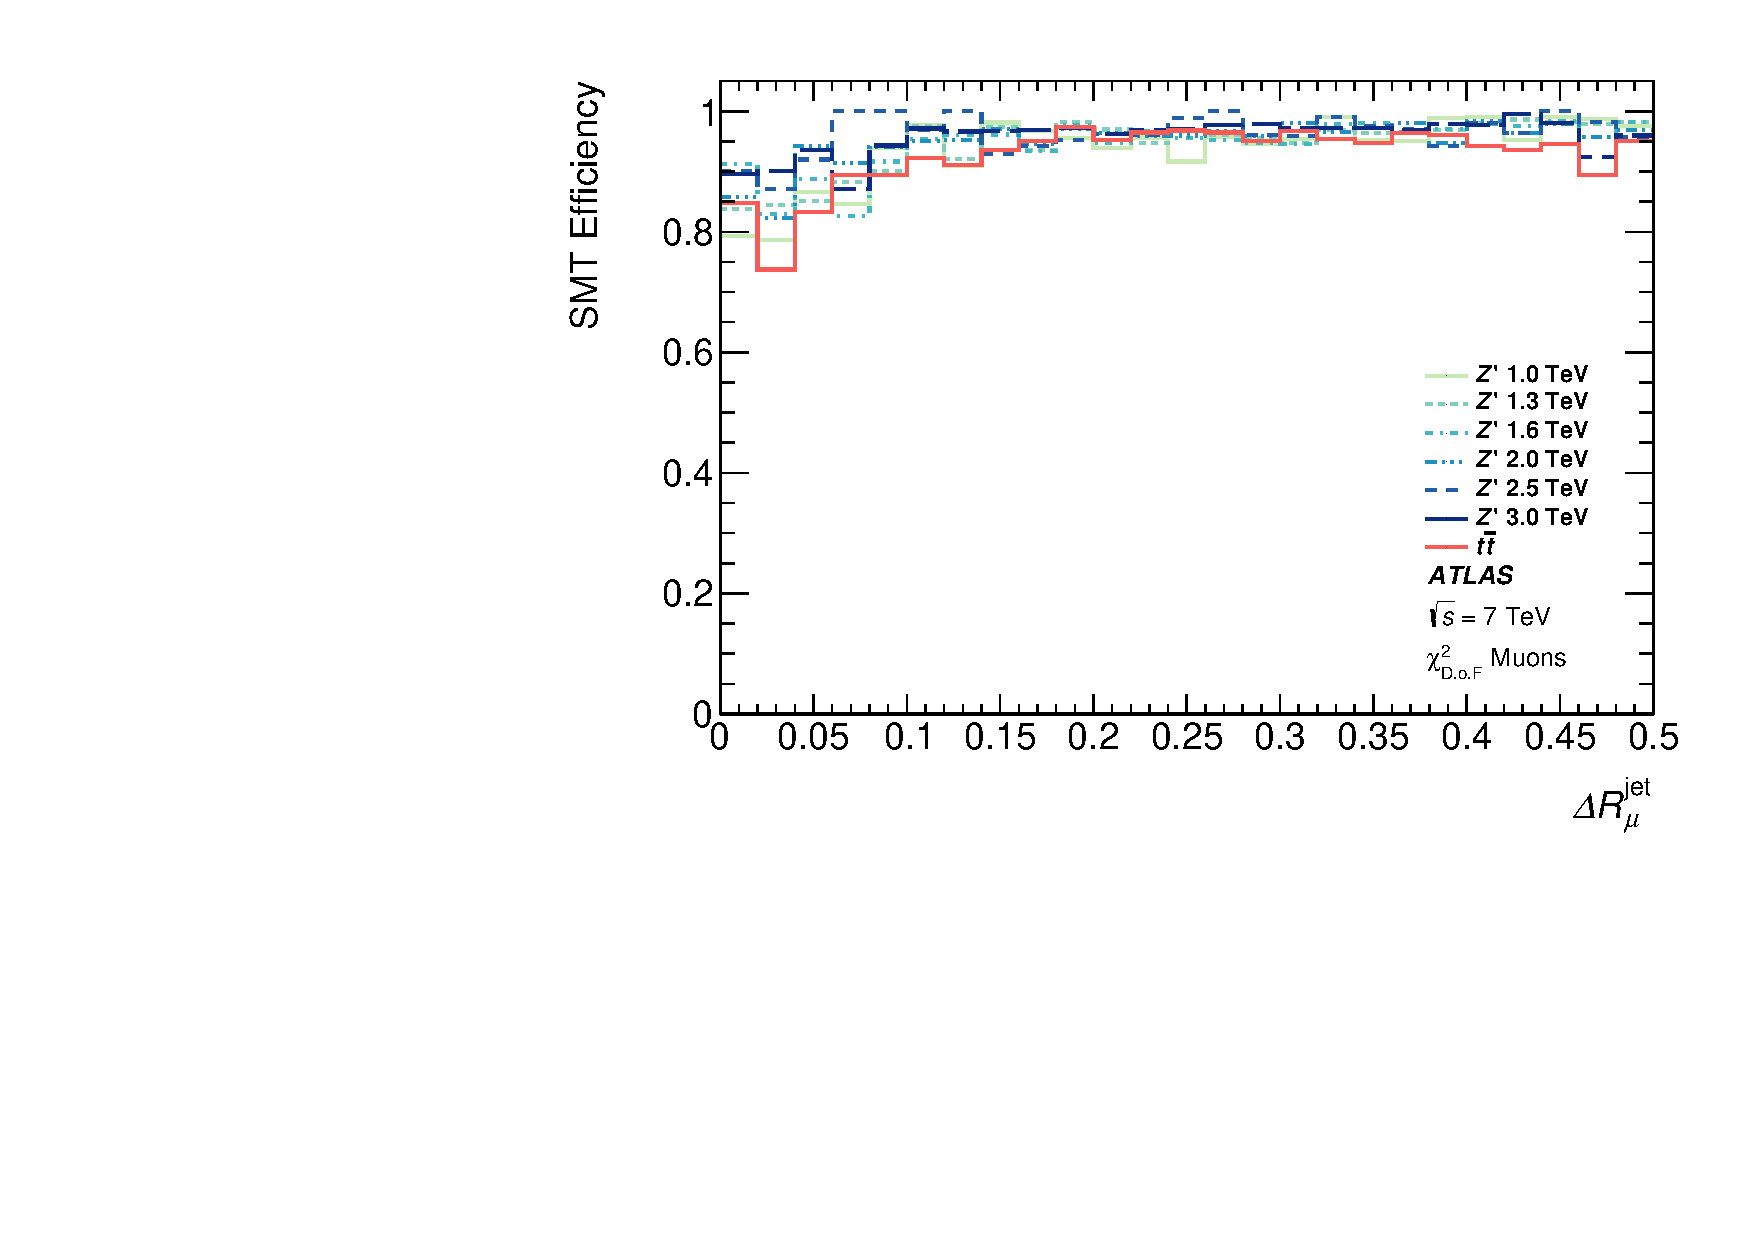
\includegraphics[width=\textwidth]{PartBoosted/Plots/he_staco_smt_dr.pdf}
    \caption{\xsm\ muon tagger}\label{fig:BoostedSMTeffVsDRmuj}
  \end{subfigure}
~%
  \begin{subfigure}{0.49\linewidth}
    \centering
    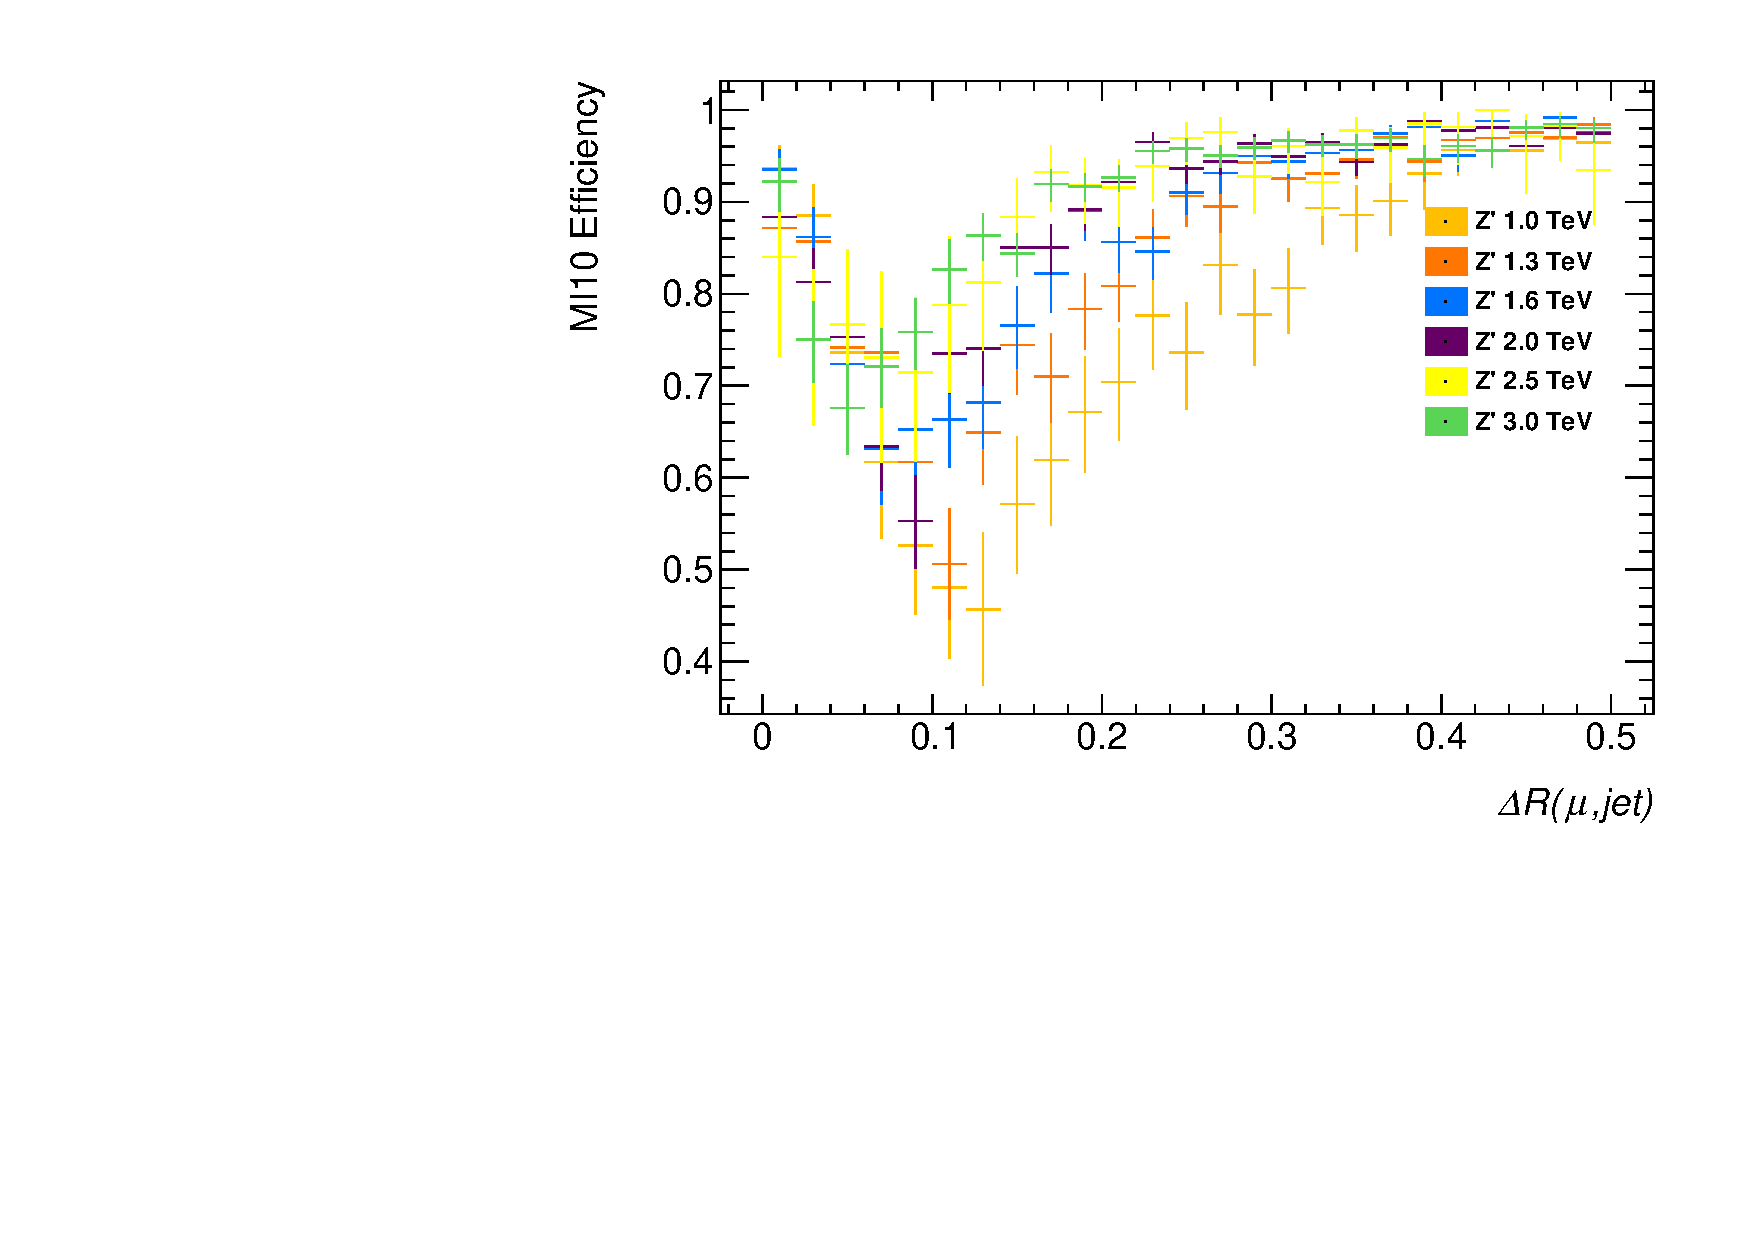
\includegraphics[width=\textwidth]{PartBoosted/Plots/he_muid_mi10_dr.pdf}
    \caption{MI10}\label{fig:BoostedMIeffVsDRmuj}
  \end{subfigure}

  \caption[Efficiency of MI10 and \xsm\ tagger as a function of the angular separation between the reconstructed muon and the nearest reconstructed jet.]{Efficiency of MI10 and \xsm\ tagger as a function of the angular separation between the reconstructed muon and the nearest reconstructed jet. Uncertainties are omitted for clarity. The dip in the MI efficiency at low $\DeltaR$ is removed in the nominal analysis by cutting at $\DeltaR<0.1$}\label{fig:BoostedEfficiencyVsDRmuj}
\end{figure}

\begin{figure}[htbp]
  \begin{subfigure}{0.49\linewidth}
    \centering
    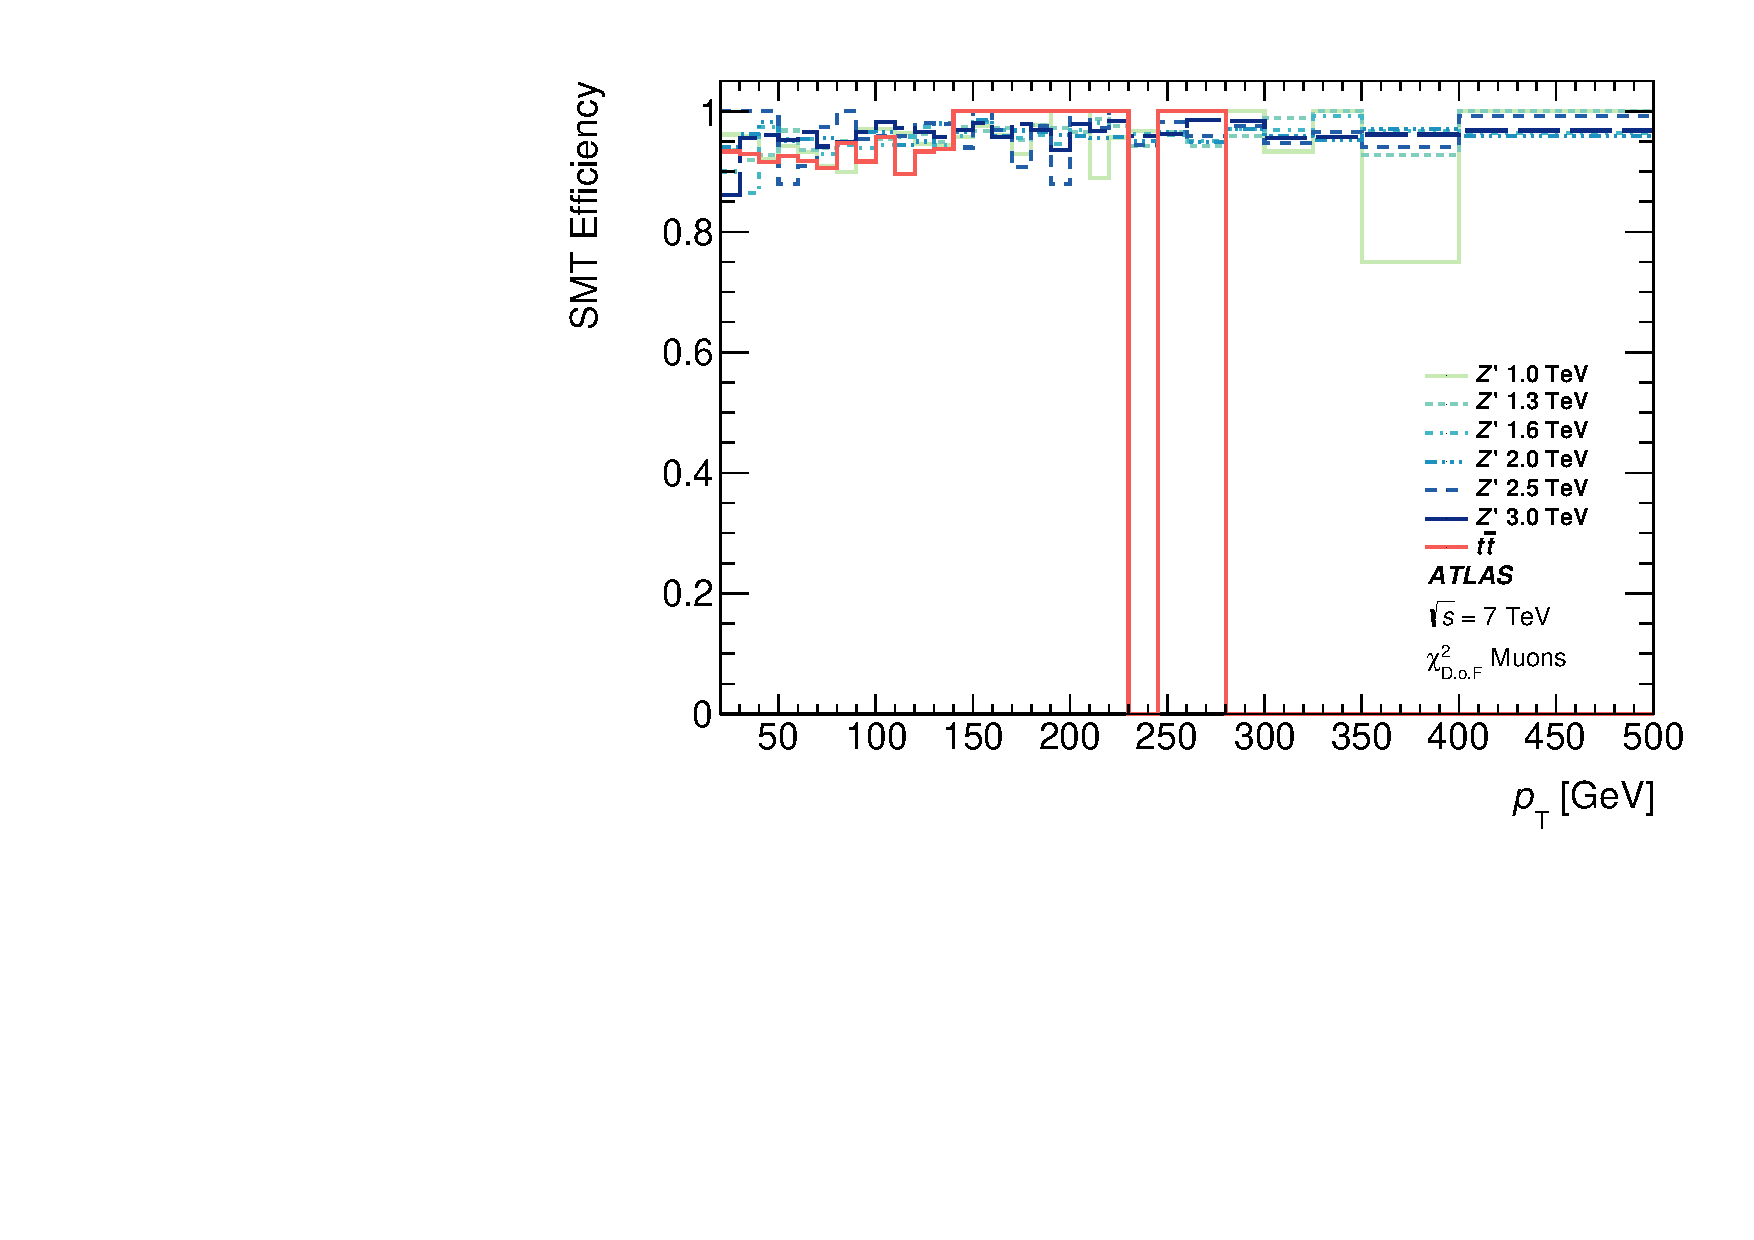
\includegraphics[width=\textwidth]{PartBoosted/Plots/he_staco_smt_pt.pdf}
    \caption{\xsm\ muon tagger}\label{fig:BoostedSMTeffVsPt}
  \end{subfigure}
~%
  \begin{subfigure}{0.49\linewidth}
    \centering
    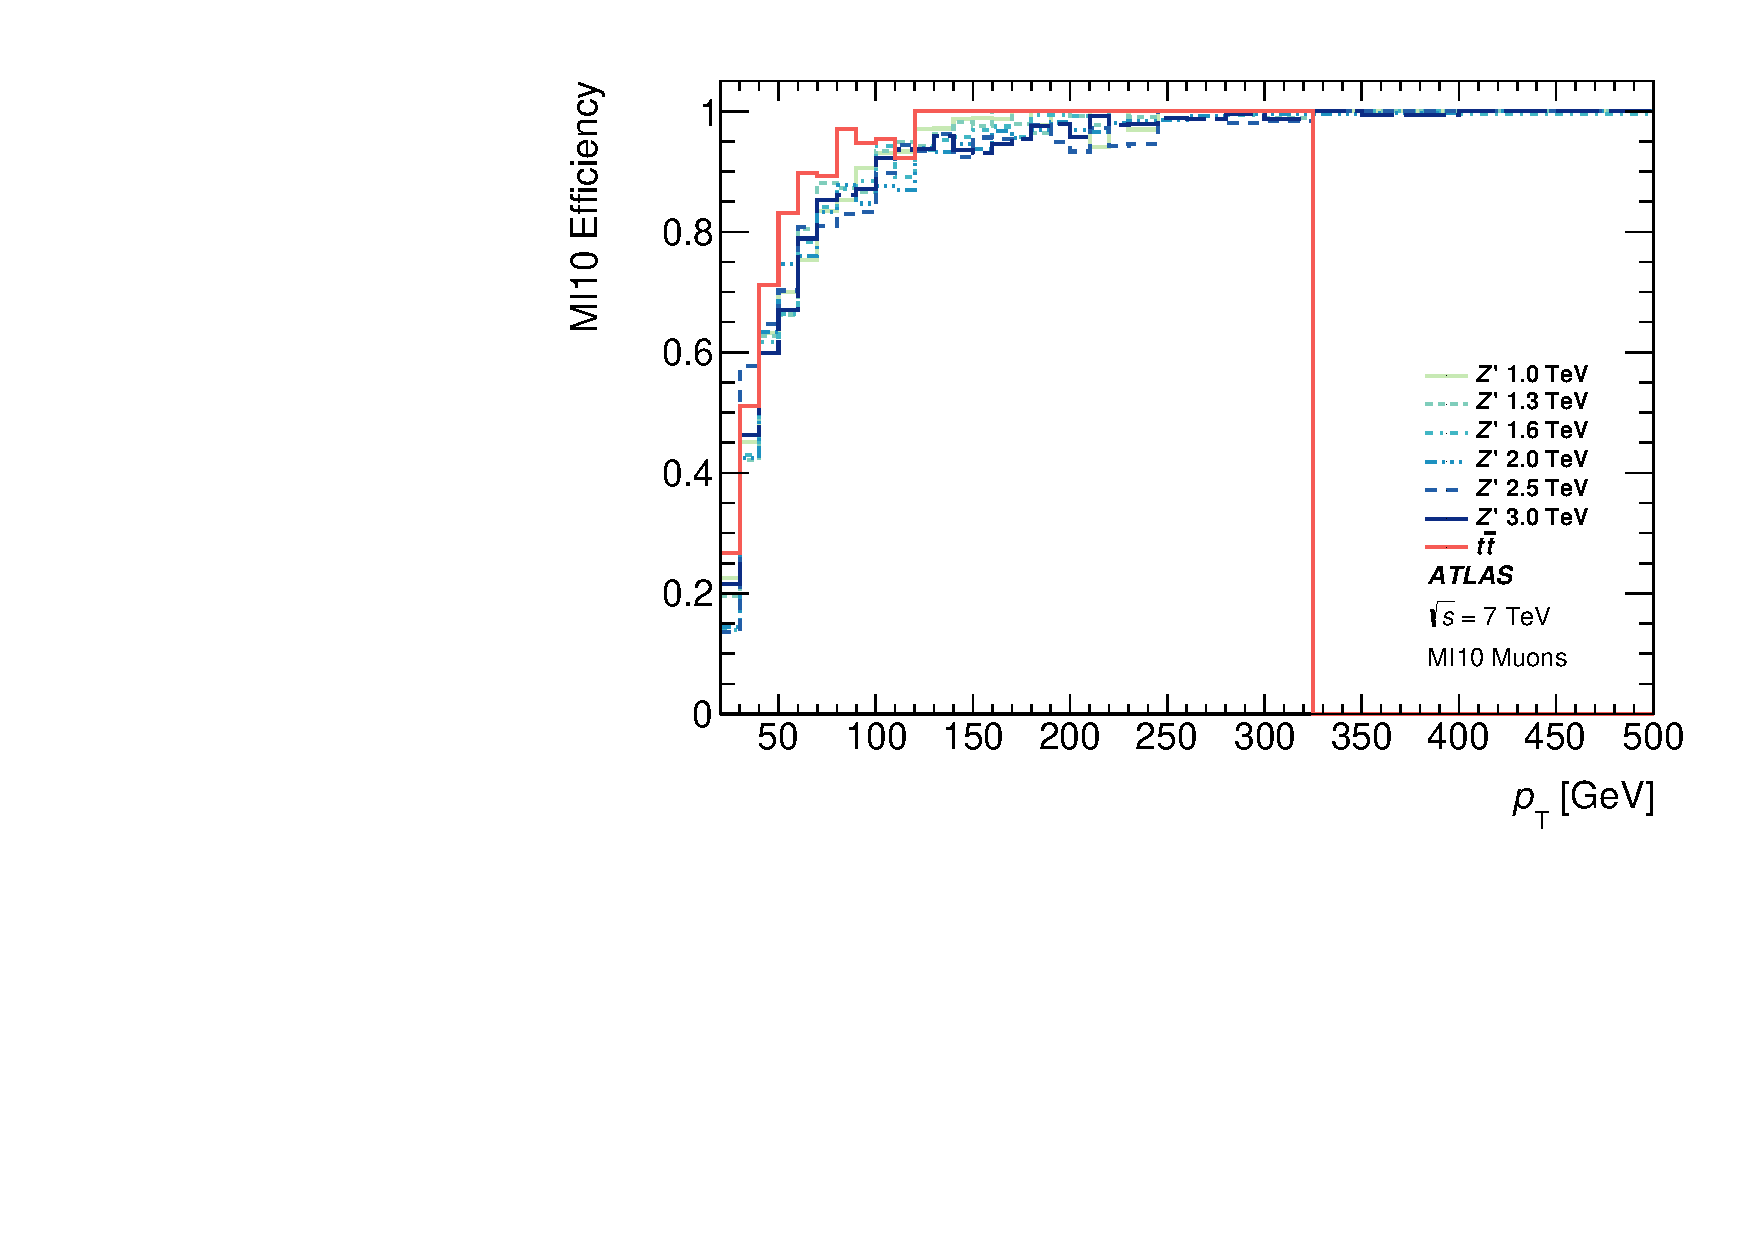
\includegraphics[width=\textwidth]{PartBoosted/Plots/he_muid_mi10_pt.pdf}
    \caption{MI10}\label{fig:BoostedMIeffVsPt}
  \end{subfigure}

  \caption{Efficiency of MI10 and the \xsm\ muon tagger as a function of the transverse momentum of the muon. Uncertainties are omitted for clarity. The missing bins are due to lack of data in that region of phase-space.}\label{fig:BoostedEfficiencyVsPt}
\end{figure}

\subsection{Background}

A preliminary estimation of the fake-rate for the \xsm\ tagger and mini-isolation in a boosted environment was carried out.

The dominant backgrounds for boosted \ttbar\ events include multijet events and SM resolved \ttbar. A measure of the acceptance of multijet background is provided here. 

This source is normally estimated using complex data-driven methods, however as this is a preliminary study, a simulated sample of all-hadronic events is used instead. The all-hadronic sample is constructed by requiring that no truth $W$ muons be present. These events do not perfectly represent the dominant multijet sources such as $b\bar{b}$ production, but the lack of a signal $W$ muon make these events a suitable preliminary substitute. 

The lack of an isolation requirement is expected to result in a substantial increase in the amount of background selected. Soft muons from the semileptonic decay of HF quarks will also be selected, this then increases acceptance to $b\bar{b}$ events.

The same efficiency definitions described in Section~\ref{sec:BoostedEfficiencyDefinition} are used here. No truth-matching is carried out here due to the lack of a $W$ muon, so only the \xsm\ tagger and mini-isolation fake rates are shown. 

As expected, MI exhibits a low fake rate while maintaining very high signal efficiency (Table~\ref{tab:BoostedBackgroundResults}) with or without overlap removal. In comparison, removing the isolation requirement entirely greatly increases the background acceptance when using the \xsm\ tagger. Introducing overlap removal does reduce the background substantially for both selections but \xsm\ fake rate remains above \SI{20}{\percent}. 

The increase in signal acceptance does not make this methodology sufficiently advantageous, particularly when considering the large increase in fake rate. An examination of the $b$-tagging potential of the \xsm\ tagger is presented in the next section.

\begin{table}[htbp]
  \centering
    \begin{tabular}{@{}
                    S[table-format=4]
                    S[table-format=2.1(1)]
                    S[table-format=1.1(1)]
                    S[table-format=2.1(2)]
                    S[table-format=1.1(1)]
                    @{}}
      \toprule
      {\mzp\ [\si{GeV}]} & \multicolumn{4}{c}{Fake rate [\si{\percent}]} \\
      \cmidrule{2-5}
      & {\eff{\textrm{\xsm}}{}} & {\eff{\textrm{MI10}}{}} & {\eff{\textrm{\xsm+overlap}}{}} & {\eff{\textrm{MI10+overlap}}{}} \\
      \midrule
      1000 & 92.8(3) & 4.1(2) & 20.8(5)  & 2.4(2)\\
      1300 & 92.4(3) & 4.8(2) & 28.9(5)  & 3.7(2)\\
      1600 & 91.6(3) & 5.5(2) & 36.9(5)  & 4.5(2)\\
      2000 & 91.1(3) & 7.1(2) & 45.5(5)  & 6.1(2)\\
      2500 & 90.1(6) & 6.4(5) & 48.7(11) & 5.6(5)\\
      3000 & 90.1(3) & 6.6(2) & 46.1(5)  & 5.7(2)\\
      \bottomrule
    \end{tabular}
    \caption{Fake rate of the \xsm\ tagger and mini-isolation with and without overlap removal as measured using all \Zprime\ mass points. The uncertainty is statistical only.}\label{tab:BoostedBackgroundResults}
\end{table}

\section{B-tagging potential in boosted events}

A study of the $b$-tagging performance of the SMT tagger was carried out and is presented here along with a comparison against the nominal MV1 tagger. The performance is estimated in simulation using the \Zprime\ samples described earlier. Using truth information, the $b$-quarks from the top decays are identified and then matched to reconstructed anti-$k_t$ jets of cone-size $\DeltaR=0.4$. The matching is done by requiring the jet and $b$-quark lie within $\DeltaR_{b}^{\textrm{jet}}<0.3$ of each other. The value of the $\DeltaR$ used here is a standard used at ATLAS for the purpose of flavour tagging of jets from simulated data. These matched jets then tentatively form a pool of jets on which the tagging performance can be measured. This matching procedure has an efficiency associated with it defined as
%
\begin{equation}
  \epsilon_{b\textrm{ to jet}} = \frac{b\textrm{ quarks with }\DeltaR_{\textrm{jet}}^{b}<\num{0.3}}{b\textrm{ quarks from }t\rightarrow Wb} \\
\end{equation}

The matching efficiency remains above \SI{80}{\percent} through-out the tested mass range (Table~\ref{tab:BoostedBJetMatching}), and there appears to be a trend of increasing matching efficiency with mass range.
%
\begin{table}
  \robustify\bfseries
  \centering
    \begin{tabular}
    {@{}
     S[table-format=4]%
     c
     *{2}{S[table-format=6]}
     c
     S[table-format=2.1(1)]
    @{}}
      \toprule
      {\mzp\ [\si{\GeV}]} & \phantom{a} & \multicolumn{2}{c}{Number of $b$-quarks from top} & \phantom{a} & {$\epsilon_{b\textrm{ to jet}}$ [\si{\percent}]} \\
      \cmidrule{3-4}
           && {In the event} & {Matched to a jet} \\
      \midrule
      1000 && 160000(400) & 133000(400) && 83.5(1) \\
      1300 && 180000(400) & 155000(400) && 85.9(1) \\ 
      1600 && 160000(400) & 140000(400) && 87.0(1) \\
      2000 && 180000(400) & 158000(400) && 87.9(1) \\ 
      2500 && 40000(200)  & 35200(200)  && 88.0(2) \\ 
      3000 && 180000(400) & 156000(400) && 86.8(1) \\
      \bottomrule
    \end{tabular}
    \caption[Summary of $b$-quark to jet matching efficiencies for all tested \Zprime\ masses.]{Summary of $b$-quark to jet matching efficiencies for all tested \Zprime\ masses. The uncertainty is statistical only.}\label{tab:BoostedBJetMatching}
\end{table}

The tagging efficiency can be defined in two ways. The first folds the effect of the low $b\rightarrow\mu$ branching ratio into the final efficiency. This makes the comparison with other taggers possible and is denoted by $\epsilon_{\textrm{Inc. SMT}}$.

The second definition separates the efficiency into two components: firstly, the jet is associated with a STACO combined muon by requiring $\DeltaR_{\textrm{jet}}^{\mu}<0.5$. The associated efficiency defined as,
\begin{equation}
    \epsilon_{\mu\textrm{-match}} = \frac{\textrm{Number of $b$-jets with an associated muon}}%
                         {\textrm{Number of $b$-jets}} \\
\end{equation}
%
and then both the muon and the jet are required to pass the SMT tagger selection. This step has an associated efficiency:
%
\begin{equation}
  \epsilon_{\textrm{SMT}} = \frac{\textrm{Number of jets/muons that pass the \xsm\ tagger selection}}%
                         {\textrm{Number of $b$-jets with an associated muon}}
\end{equation}

The second definition provides a more apt description of the performance of the SMT tagger but makes comparisons with other taggers incorrect. The former definition of the efficiency is used here to allow for a proper comparison between the MV1 and SMT taggers.

As expected, as the boost increases the distance between the muon and the jet decreases as shown in Table~\ref{tab:BoostedMatchingMuonToJet}. This leads to an increase in the muon-to-jet matching efficiency.

\begin{table}[htbp]
  \centering
    \begin{tabular}{@{}
                    S[table-format=4]
                    S[table-format=5(3)]
                    S[table-format=2.1(1)]
                    @{}}
      \toprule
      {\mzp\ [\si{\GeV}]} & {Jets matched to muon} & {$\epsilon_{\mu\textrm{-match}}$ [\si{\percent}]} \\
      \midrule
      1000 & 22100(100) & 17.1(3) \\
      1300 & 28400(200) & 18.2(2) \\
      1600 & 27600(200) & 20.4(2) \\
      2000 & 33500(200) & 20.7(2) \\
      2500 & 7540(90)   & 21.2(5) \\
      3000 & 32800(200) & 21.5(2) \\
      \bottomrule
    \end{tabular}
    \caption{Results of the muon to jet association in MC simulated inclusive \Zprime\ samples.}\label{tab:BoostedMatchingMuonToJet}
\end{table}

The tagging yields as well as the overlap yield between the taggers are shown in Table~\ref{tab:BoostedSummaryBtaggingEff}. As expected the MV1 tagger selects the vast majority of the $b$-jets while the effect of the semileptonic $b$-decay is also noted in the lower SMT yields.

The SMT tagging efficiency appears to increase with \mzp\ as shown in Table~\ref{tab:BoostedBTagEffs}. Interestingly, the performance of the MV1 tagger degrades substantially with increasing \mzp\ mass. Also note that the overlap between the MV1 tagger and the SMT tagger decreases with \mzp. This means that using the SMT tagger alongside the MV1 tagger can provide substantial increases in yields at higher \Zprime\ masses.

\begin{table}[htbp] 
  \centering
    \begin{tabular}{@{}%
                    S[table-format=4(3)] % Mass Label
                    S[table-format=5(3)] % SMT Yield
                    S[table-format=6(3)] % MV1 Yield
                    S[table-format=5(3)] % Both Yield
                    @{}}
      \toprule
      {\mzp\ [\si{\GeV}]} & \multicolumn{3}{c}{Number of jets tagged by} \\
      \cmidrule{2-4}
           & {SMT}  & {MV1}  & {Both} \\
      \midrule
      1000 & 19600(100) & 96900(300)  & 14800(100) \\
      1300 & 25000(200) & 109000(300) & 18100(100) \\
      1600 & 23900(200) & 93100(300)  & 16300(100) \\
      2000 & 28300(200) & 96200(300)  & 17800(100) \\
      2500 & 6250(80)   & 19800(100)  & 3690(60)   \\
      3000 & 27200(200) & 89400(300)  & 16200(100) \\
      \bottomrule
    \end{tabular}
    \caption[Results of the $b$-jet tagging study. Shown are the number of jets tagged by the SMT tagger, the MV1 tagger, and both.]{Results of the $b$-jet tagging study. Shown are the number of jets tagged by the SMT tagger, the MV1 tagger, and both. These jets have been truth-matched to $b$-quarks.}\label{tab:BoostedSummaryBtaggingEff}
\end{table}

\begin{table}[htbp]
  \centering
    \begin{tabular}{@{}
                    S[table-format=4] % Mass Label
                    *{3}{S[table-format=2.1(1)]} % SMT Efficiency
                    S[table-format=2] % Added Acceptance
                    @{}}
      \toprule
      {\mzp\ [\si{\GeV}]} & {$\epsilon_{\textrm{SMT}}$ [\si{\percent}]} & {$\epsilon_{\textrm{MV1}}$ [\si{\percent}]} & {Overlap [\si{\percent}]} & {Added Acceptance [\si{\percent}]} \\ 
      \midrule
      1000 & 14.7(1) & 72.7(1) & 75.3(1) & 5  \\
      1300 & 16.2(1) & 70.7(1) & 72.4(1) & 6  \\
      1600 & 17.2(1) & 66.9(1) & 68.0(1) & 8  \\
      2000 & 17.9(1) & 60.9(1) & 63.0(1) & 11 \\
      2500 & 17.8(2) & 56.3(2) & 59.0(2) & 13 \\
      3000 & 17.4(1) & 57.3(1) & 60.0(1) & 12 \\
      \bottomrule
    \end{tabular}
    \caption[Results of the $b$-tagging efficiency estimation for the MV1 and SMT taggers.]{Results of the $b$-tagging efficiency estimation for the MV1 and SMT taggers. The amount of overlap is shown out of the SMT tagged jets, while the added acceptance is measured as the number of jets tagged only by SMT over the number of MV1 tagged jets. The uncertainties are statistical only.}\label{tab:BoostedBTagEffs}
\end{table}

The efficiency for both taggers as a function of the jet \pt\ is shown in Figure~\ref{fig:BoostedBTaggEffs}. The performance of the MV1 tagger is clearly \pt\ dependant while the SMT tagger is more stable with respect to jet \pt. The performance of the MV1 tagger is lower at both extremes of the momentum distribution. At low jet \pt\ the performance of secondary vertex reconstruction is degraded due to the lower decay length. In contrast, at high jet \pt\ the primary source of $b$-tagging efficiency loss comes from the shift in the jet axis away from the the $B$-hadron direction. If the shift is very large, some of the $B$-hadron components may not be associated with the jet and not enter into the discriminants that make up the MV1 tagger~\cite{Boosted:MV1TaggerHighPt}.

\begin{figure}[tbhp]
  \centering
  \begin{subfigure}[b]{0.75\textwidth}
    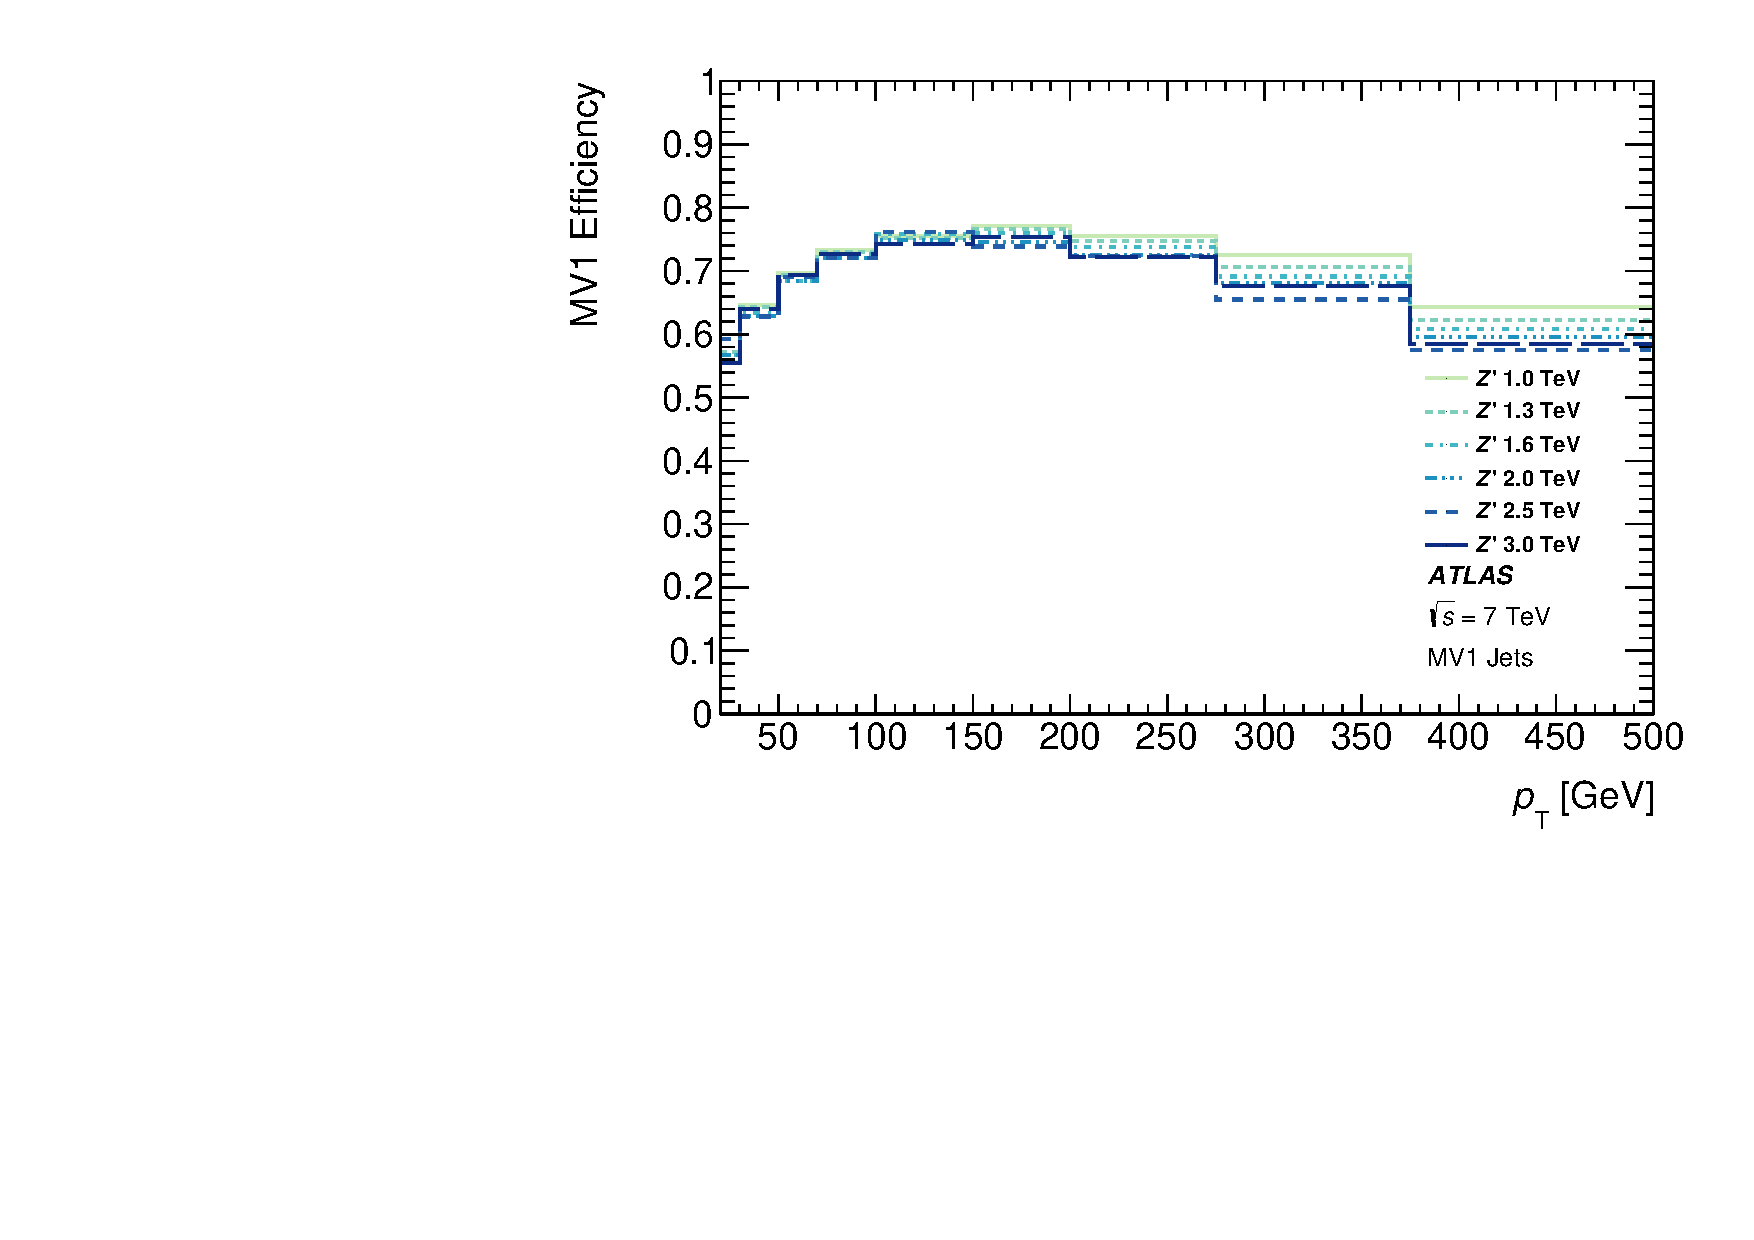
\includegraphics[width=\textwidth]{PartBoosted/Plots/he_mv1_jet_pt.pdf}
    \caption{MV1 Tagger}\label{fig:BoostedBTaggMV1}
  \end{subfigure}
  
  \begin{subfigure}[b]{0.75\textwidth}
    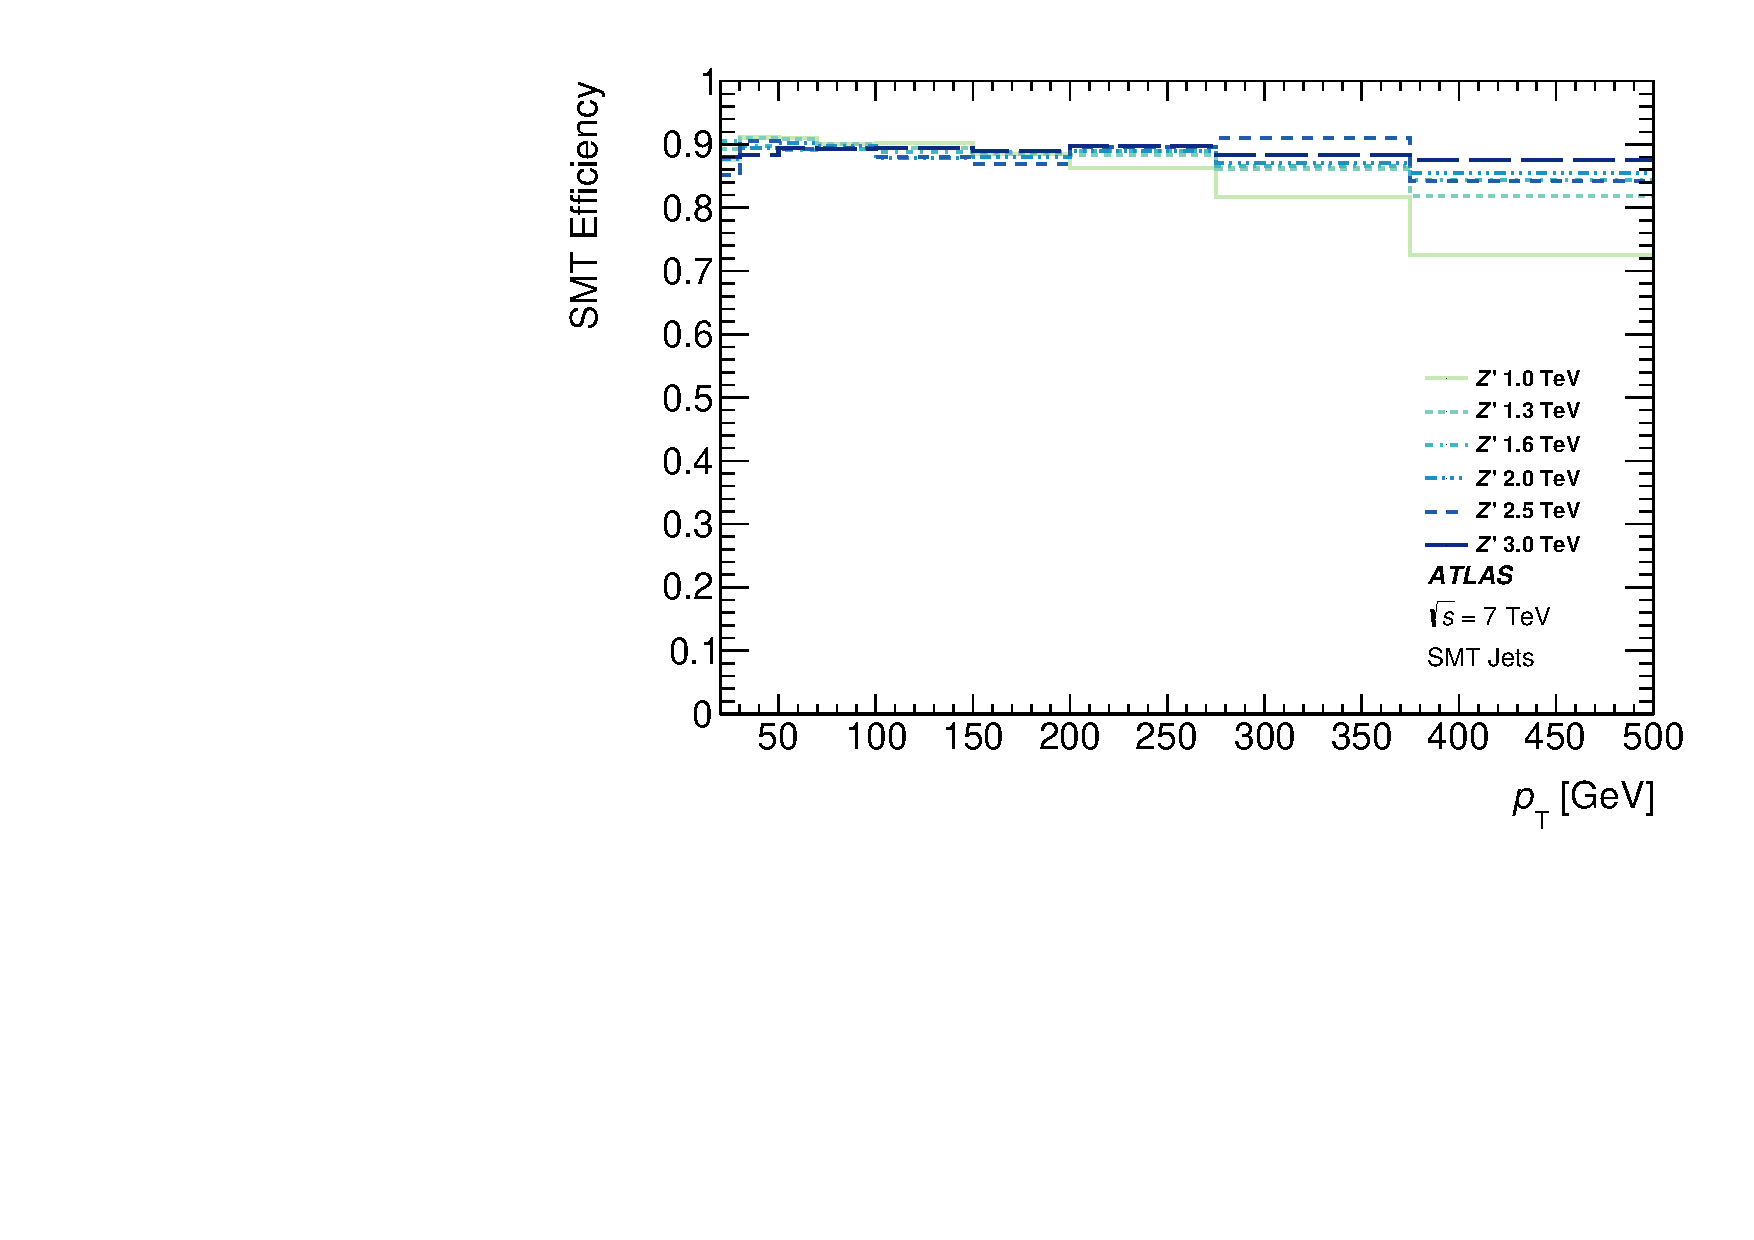
\includegraphics[width=\textwidth]{PartBoosted/Plots/he_smt_jet_pt.pdf}
    \caption{SMT Tagger}\label{fig:BoostedBTaggSMT}
  \end{subfigure}
  \caption{The $b$-tagging efficiency distributions as a function of jet \pt\ for the MV1 tagger and the SMT tagger as measured in all \Zprime\ mass points.}\label{fig:BoostedBTaggEffs}
\end{figure}

The performance of the SMT tagger in a boosted environment looks promising from this preliminary study, however a more careful measurement of the performance needs to be conducted. In addition, it is important to also perform a fake-rate study in such a boosted environment. As was observed in the calibration of the tagger on both 2012 and 2011 data, the efficiency of tagging a soft muon is not affected by the isolation of that muon.
